\chapter{多类疾病标记物定位的实验评估}\label{sec:multi_classes}
在上一章中,与CAM和Grad-CAM相比,本文通过在两个数据集上的实验结果说明了本文提出的模型在处理二类疾病标记物定位问题时的优异表现。本章将本文提出的模型由二类问题推广到多类问题。首先在\ref{sec:mul_classes_ds_intro}小节中,本文将会介绍本章实验数据集。在\ref{sec:multi_classes_experiment_setting}小节中,本文将会说明实验相关设置。从\ref{sec:multi_classes_experiments_res}小节开始,本文将展示本文提出的模型在处理多类疾病标记物定位任务上的实验结果。最后本文会在\ref{sec:multi_classes_hyper_paras}小节中对超参数$\lambda_{1}$和$\lambda_{2}$组合进行相关测试。
\section{数据集介绍}\label{sec:mul_classes_ds_intro}
\subsection{多类模拟皮肤病病变数据集}
多类模拟皮肤病病变数据集同样是包含人工疾病标记物的皮肤图像,图像尺寸大小均为$128\times 128$,图像均以PNG格式存储,每张图像不仅有图像级标注,还有像素级标注,故可用于定量分析有关的实验评估。在\ref{subsec:bin_simulated_skin_ds}小节中用到的二类模拟皮肤病病变数据集基础上额外增加了两类,故多类模拟皮肤病病变数据集中一共有$4$类,其中$3$类异常,$1$类正常。正常类图像是从ISIC2018~\cite{codella2019skin, tschandl2018ham10000}分类任务中的图像\footnote{https://challenge2018.isic-archive.com/task3/}通过滑动窗口方式收集$922$张正常皮肤图像(实际上是图像块)。本章将带有Image-Net缩略图(疾病标记物)的异常图像叫做第一类异常,第一类异常与二类模拟皮肤病病变数据集中的异常类一样,生成过程也相同。本章将带有黑色素瘤病变区域(疾病标记物)的异常图像叫做第二类异常,为了生成第二类异常,我们首先从ISIC2018分类任务提供的数据集(注意没有重复使用图像)中提取了图像大小为$128\times 128$的正常图像(同样通过滑动窗口方式)。同时,我们根据ISIC2018的分割任务\footnote{https://challenge2018.isic-archive.com/task1/}中的预训练分割模型,将其中的黑素瘤像素区域提取出来并嵌入到正常图像中。在此过程中,为了模拟真实皮肤图像中疾病标记物的数量、大小和所在位置的随机变化,我们通过随机参数控制,在每个模拟皮肤图像的一定范围内随机生成这些参数的值。具体来说,黑色素瘤病变区域尺寸大小为$2\times 2$、$5\times 5$、$8\times 8$或者$16\times 16$。另外,为了产生不规则形状的疾病标记物,对于黑色素瘤区域中的每个像素,以$1/3$概率稀疏。我们还设置每张正常图像中嵌入的黑色素瘤区域的数量不同($1$到$4$个不等)。第三类异常图像与第一类异常图像生成方法相同,只是第三类异常图像中的疾病标记物不再是Image-Net图像的缩略图,而是圆环。注意,为了保证三类异常图像中模拟疾病标记物的真实性,我们同样对第三类异常图像进行了局部模糊。最终,正常类、第一类异常、第二类异常和第三类异常分别有$922$、$1,310$、$1,051$、$1,062$张样本。该数据集中的部分图像示例如图\ref{fig:mul_classes_simulated_ds}所示,按照从上到下,从左到右的顺序,图中第$1$行第$1$列到第$1$行第$4$列为第一类异常;第$1$行第$5$列到第$1$行第$8$列为第二类异常;第$2$行第$1$列到第$2$行第$4$列为第三类异常;第$2$行第$5$列到第$2$行第$8$列为正常图像。
\begin{figure}[h]
	\centering
	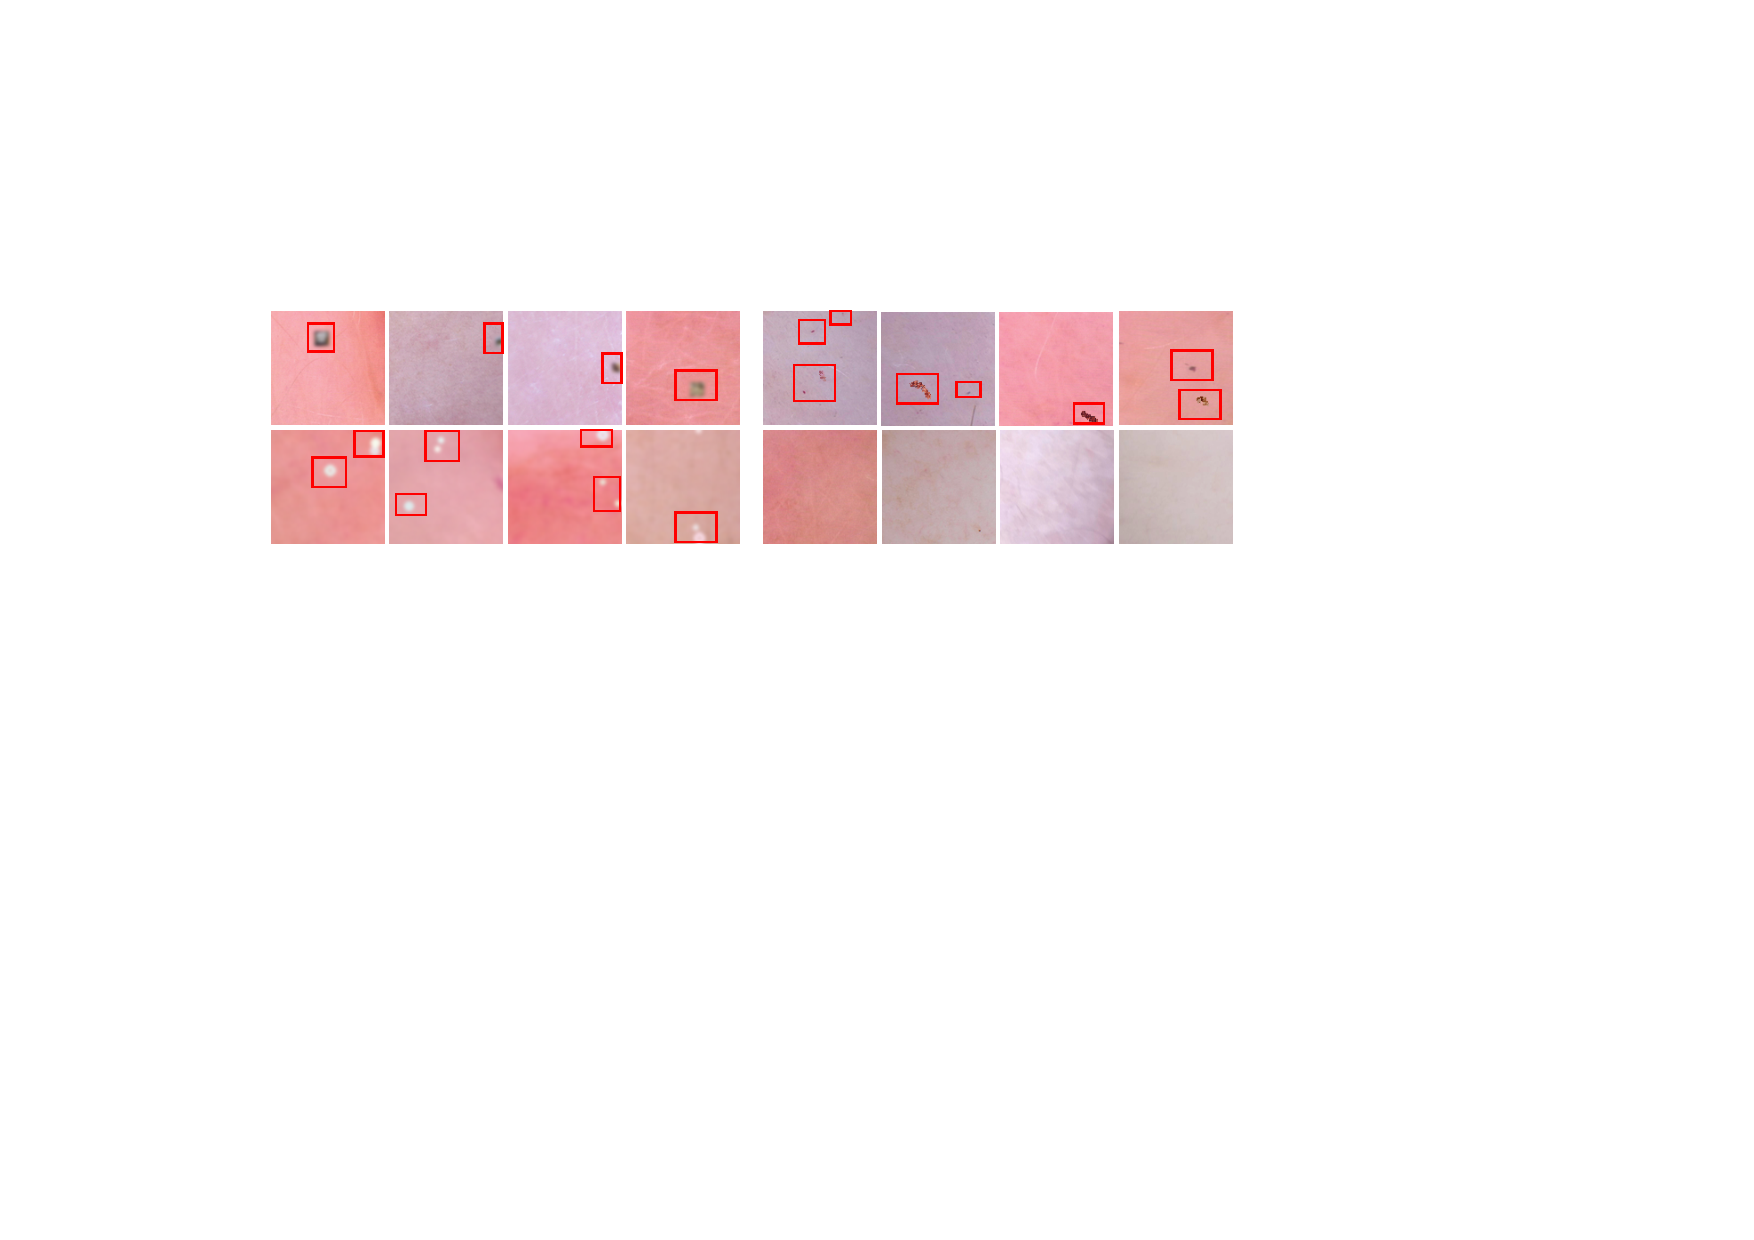
\includegraphics[width=1.0\textwidth]{figure/multi_classes_simulated_skin.pdf}
	\caption[多类模拟皮肤病病变数据集部分图像示例]{多类模拟皮肤病病变数据集部分图像示例(红色矩形框表示疾病标记物)。}
	\label{fig:mul_classes_simulated_ds}
\end{figure}
\vspace{-0.7cm}
\section{评价标准与实验设置}
\subsection{评价标准}
同样由于多类模拟皮肤病病变数据集中三个异常类的正负像素比例十分悬殊(见表\ref{tab:multi_ds_pixel_freqs}),所以本章评价标准与上一章相同,采用P-R曲线及其AUC评价不同方法定位疾病标记物的性能。与上一章不同的是,为了衡量GAN中的编码器-解码器对正常图像的保持能力和对异常图像的转化能力,本章将自定义评价指标。
\begin{table}[h]
	\centering
	\caption[多类模拟皮肤病病变数据集上三类异常图像正负像素数量统计表]{多类模拟皮肤病病变数据集上三类异常图像正负像素数量统计表。}
	\label{tab:multi_ds_pixel_freqs}
	\begin{tabular}{c|c|c|c}
		\toprule[2pt]
		数据集名称 & 正常像素数量 & 异常像素数量 & 比例 \\
		\midrule[2pt]
		第一类异常&  $21,222,487$ & $240,553$ & $\simeq 88: 1$ \\ \hline
		第二类异常&  $17,129,210$ & $90,374$ & $\simeq 190: 1$ \\ \hline
		第三类异常 & $17,341,855$ & $57,953$ & $\simeq 299: 1$ \\
		\bottomrule[2pt]
	\end{tabular}
\end{table}
\vspace{-0.7cm}
\subsection{实验设置}\label{sec:multi_classes_experiment_setting}
与上一章中二类问题所采用的实验设置相比,超参数$\lambda_{1}$和$\lambda_{2}$的取值分别为$4.0$和$20.0$,每次迭代选取$30$张图像。优化器、学习率、梯度惩罚项权重、模型迭代次数、训练集和验证集设置、预处理、是否采用数据增广等设置均与上一章相同。

训练GAN时通常每次只会送入一类正常图像和一类异常图像。而多类问题中有多个异常类,因此在处理多类问题时,一种处理方式是引入多个GAN,每个GAN都进行一类正常和一类异常的对抗学习,但是这种方式会大大增加训练模型时的复杂程度。为了避免额外引入GAN,我们将所有异常类看做一个整体,同时取样时保证所有异常图像的数量和正常图像数量相等。对于CNN分类器,我们直接将原来的二分类扩展到多分类,增加CNN分类器最后一个全连接层的输出维度,同时用多类交叉熵取代二类交叉熵损失函数。除此之外,本文提出的模型的其他结构均与上一章相同。本章中编码器-解码器也是在数据集上先进行预训练。
\section{在多类模拟皮肤病病变数据集上的疾病标记物定位}\label{sec:multi_classes_experiments_res}
本小节将展示本文提出的模型在多类模拟皮肤病病变数据集上的实验结果,本文提出的模型将与两种CNN可视化方法(CAM和Grad-CAM)作定性分析和定量分析。

与上一章相同,我们先训练得到了一个ResNet-18分类器,分类器最终的分类准确率达到了$99.9\%$,从而保证ResNet-18本身良好的分类性能。随后,与\ref{sec:bin_dr_ds_experiment}小节一样,我们分别使用CAM、Grad-CAM在多类模拟皮肤病病变数据集上完成了疾病标记物的定位任务。实验结果如图\ref{fig:multi_simulated_skin_res}所示。
\begin{figure}[h]
	\centering
	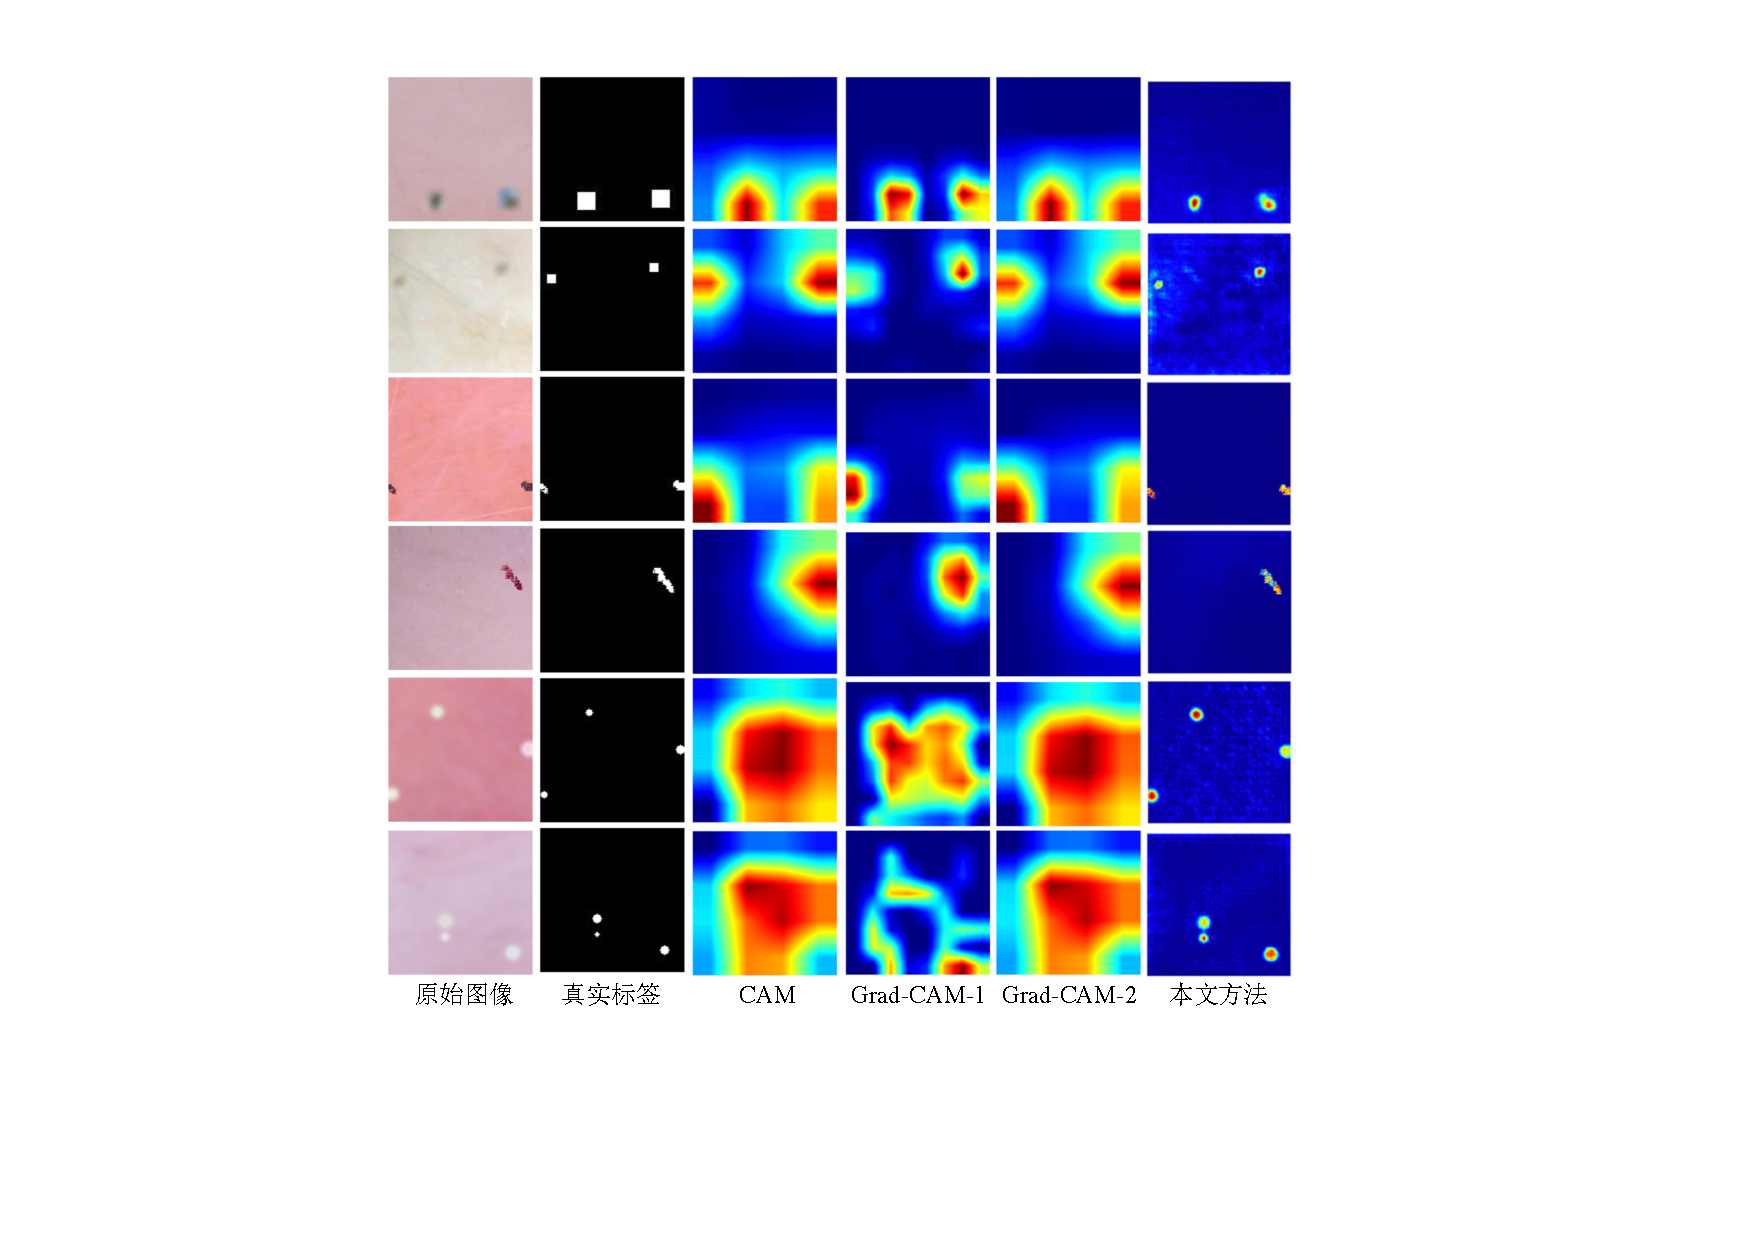
\includegraphics[width=0.975\textwidth]{figure/multi_simulated_skin_res.pdf}
	\caption[在多类模拟皮肤病病变数据集上疾病标记物定位热图对比]{在多类模拟皮肤病病变数据集上疾病标记物定位热图对比。}
	\label{fig:multi_simulated_skin_res}
\end{figure}

如图\ref{fig:multi_simulated_skin_res}所示,第$1-2$行、第$3-4$行和第$5-6$行分别为第一类异常图像、第二类异常图像和第三类异常图像的定位热图。第$1$列表示原始图像,第$2$列表示原始图像对应的像素级标签。第$3$列表示利用CAM可视化得到的定位热图,第$4$列表示利用Grad-CAM可视化中间卷积层的特征输出得到的定位热图(Grad-CAM-1),第$5$列表示Grad-CAM可视化最后一层卷积层的特征输出得到的定位热图(Grad-CAM-2),第$6$列表示本文提出的模型的定位热图。我们不难从\ref{fig:multi_simulated_skin_res}看出,第$3$列和第$5$列的定位结果相差不大,标出的异常也区域最多,虽然包括了潜在的疾病标记物,但是同时也将周边大量正常区域也误认作疾病标记物,这是因为这两种可视化方法定位疾病标记物时均需要对特征图过度上采样($4\times 4\rightarrow 128\times 128$),而Grad-CAM-1的可视化结果更为精确,也是因为中间层特征图的分辨率较高,上采样倍数较小。Grad-CAM作为CAM的扩展,对可视化层的选择更为灵活。可以发现,Grad-CAM-1取得了较为精确的结果,证明了其优于CAM的性能。相比于CAM和Grad-CAM,对于分布广泛、形状各异的疾病标记物,本文提出的模型给出了更为精确、近乎完美地定位了异常图像中的疾病标记物(第$6$列),这说明了本文提出的方法的性能优越性。

除了以上定性分析外,本小节还从定量分析角度证明了上述结论。三种方法在第一类异常、第二类异常和第三类异常图像上的P-R曲线分别如图\ref{fig:multi_simulate_pr_curve_image_net}、图\ref{fig:multi_simulate_pr_curve_skin}和图\ref{fig:multi_simulate_pr_curve_circle}所示。
\begin{figure}[H]
	\centering
	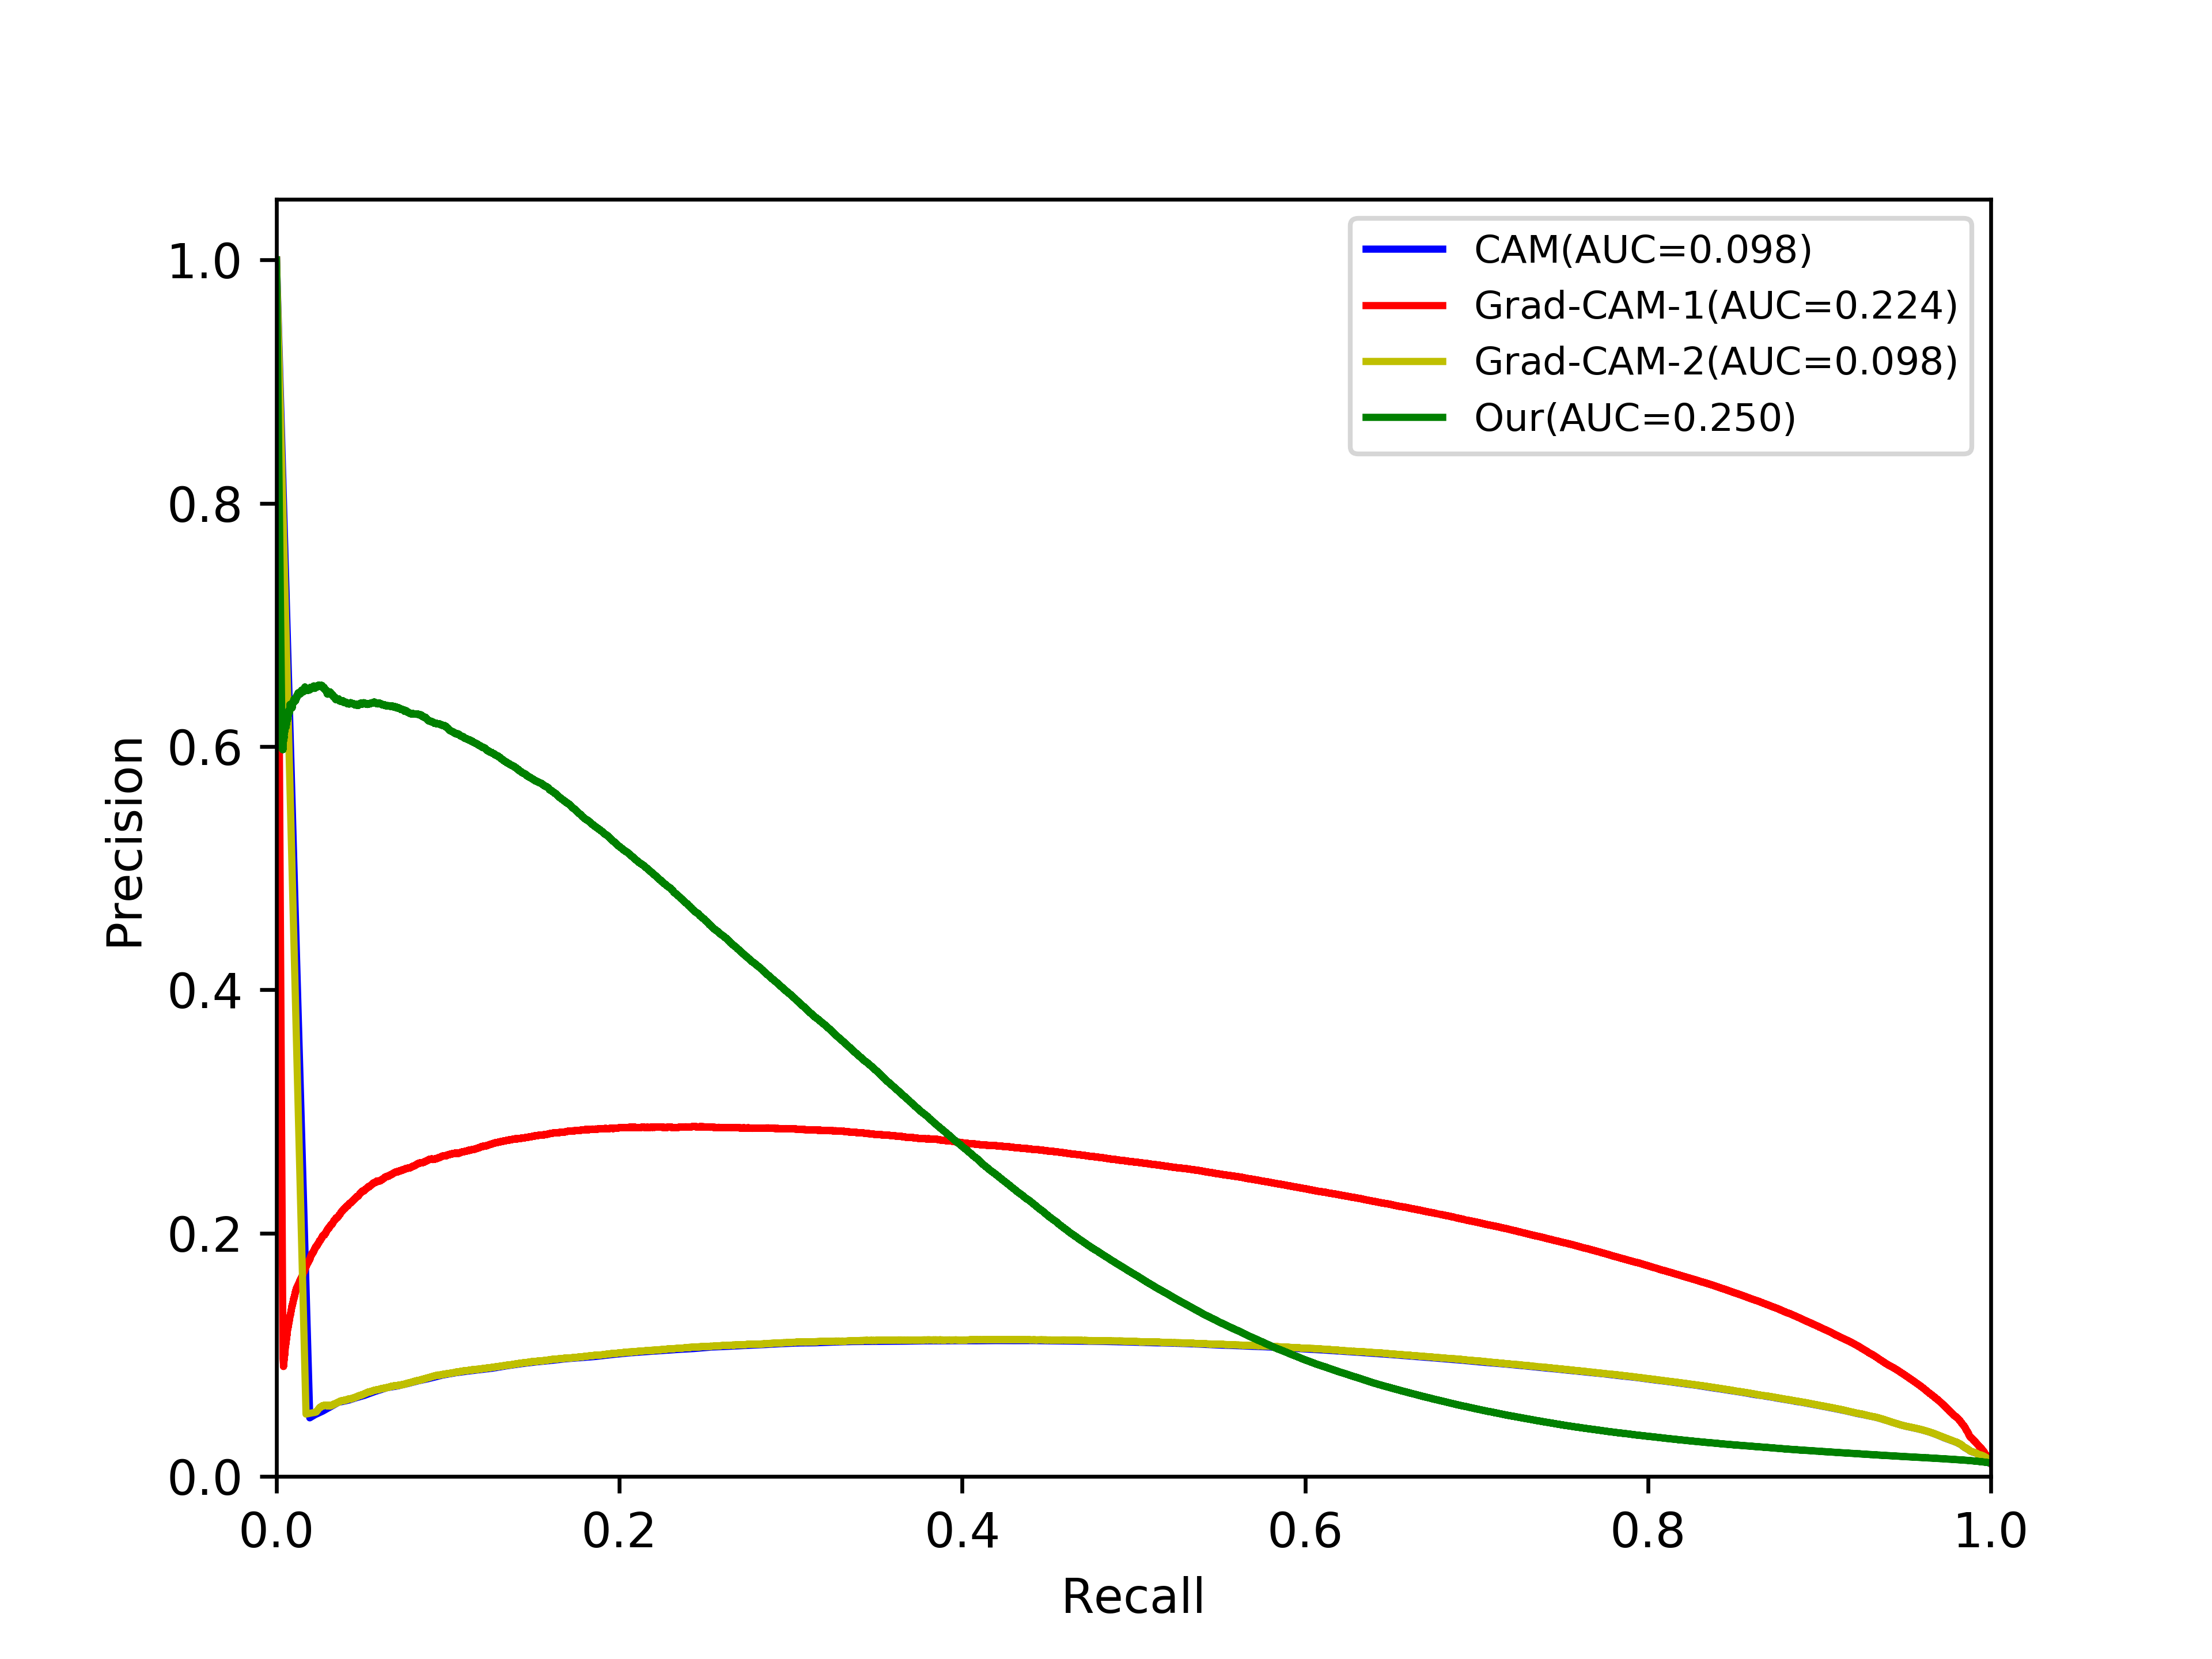
\includegraphics[width=0.6\textwidth]{figure/pr_curve_multi_skin/IMAGE_NET_pr_curve.png}
	\caption[第一类异常图像上P-R曲线对比]{第一类异常图像上P-R曲线对比。} 
	\label{fig:multi_simulate_pr_curve_image_net}
\end{figure}
\begin{figure}[H]
	\centering
	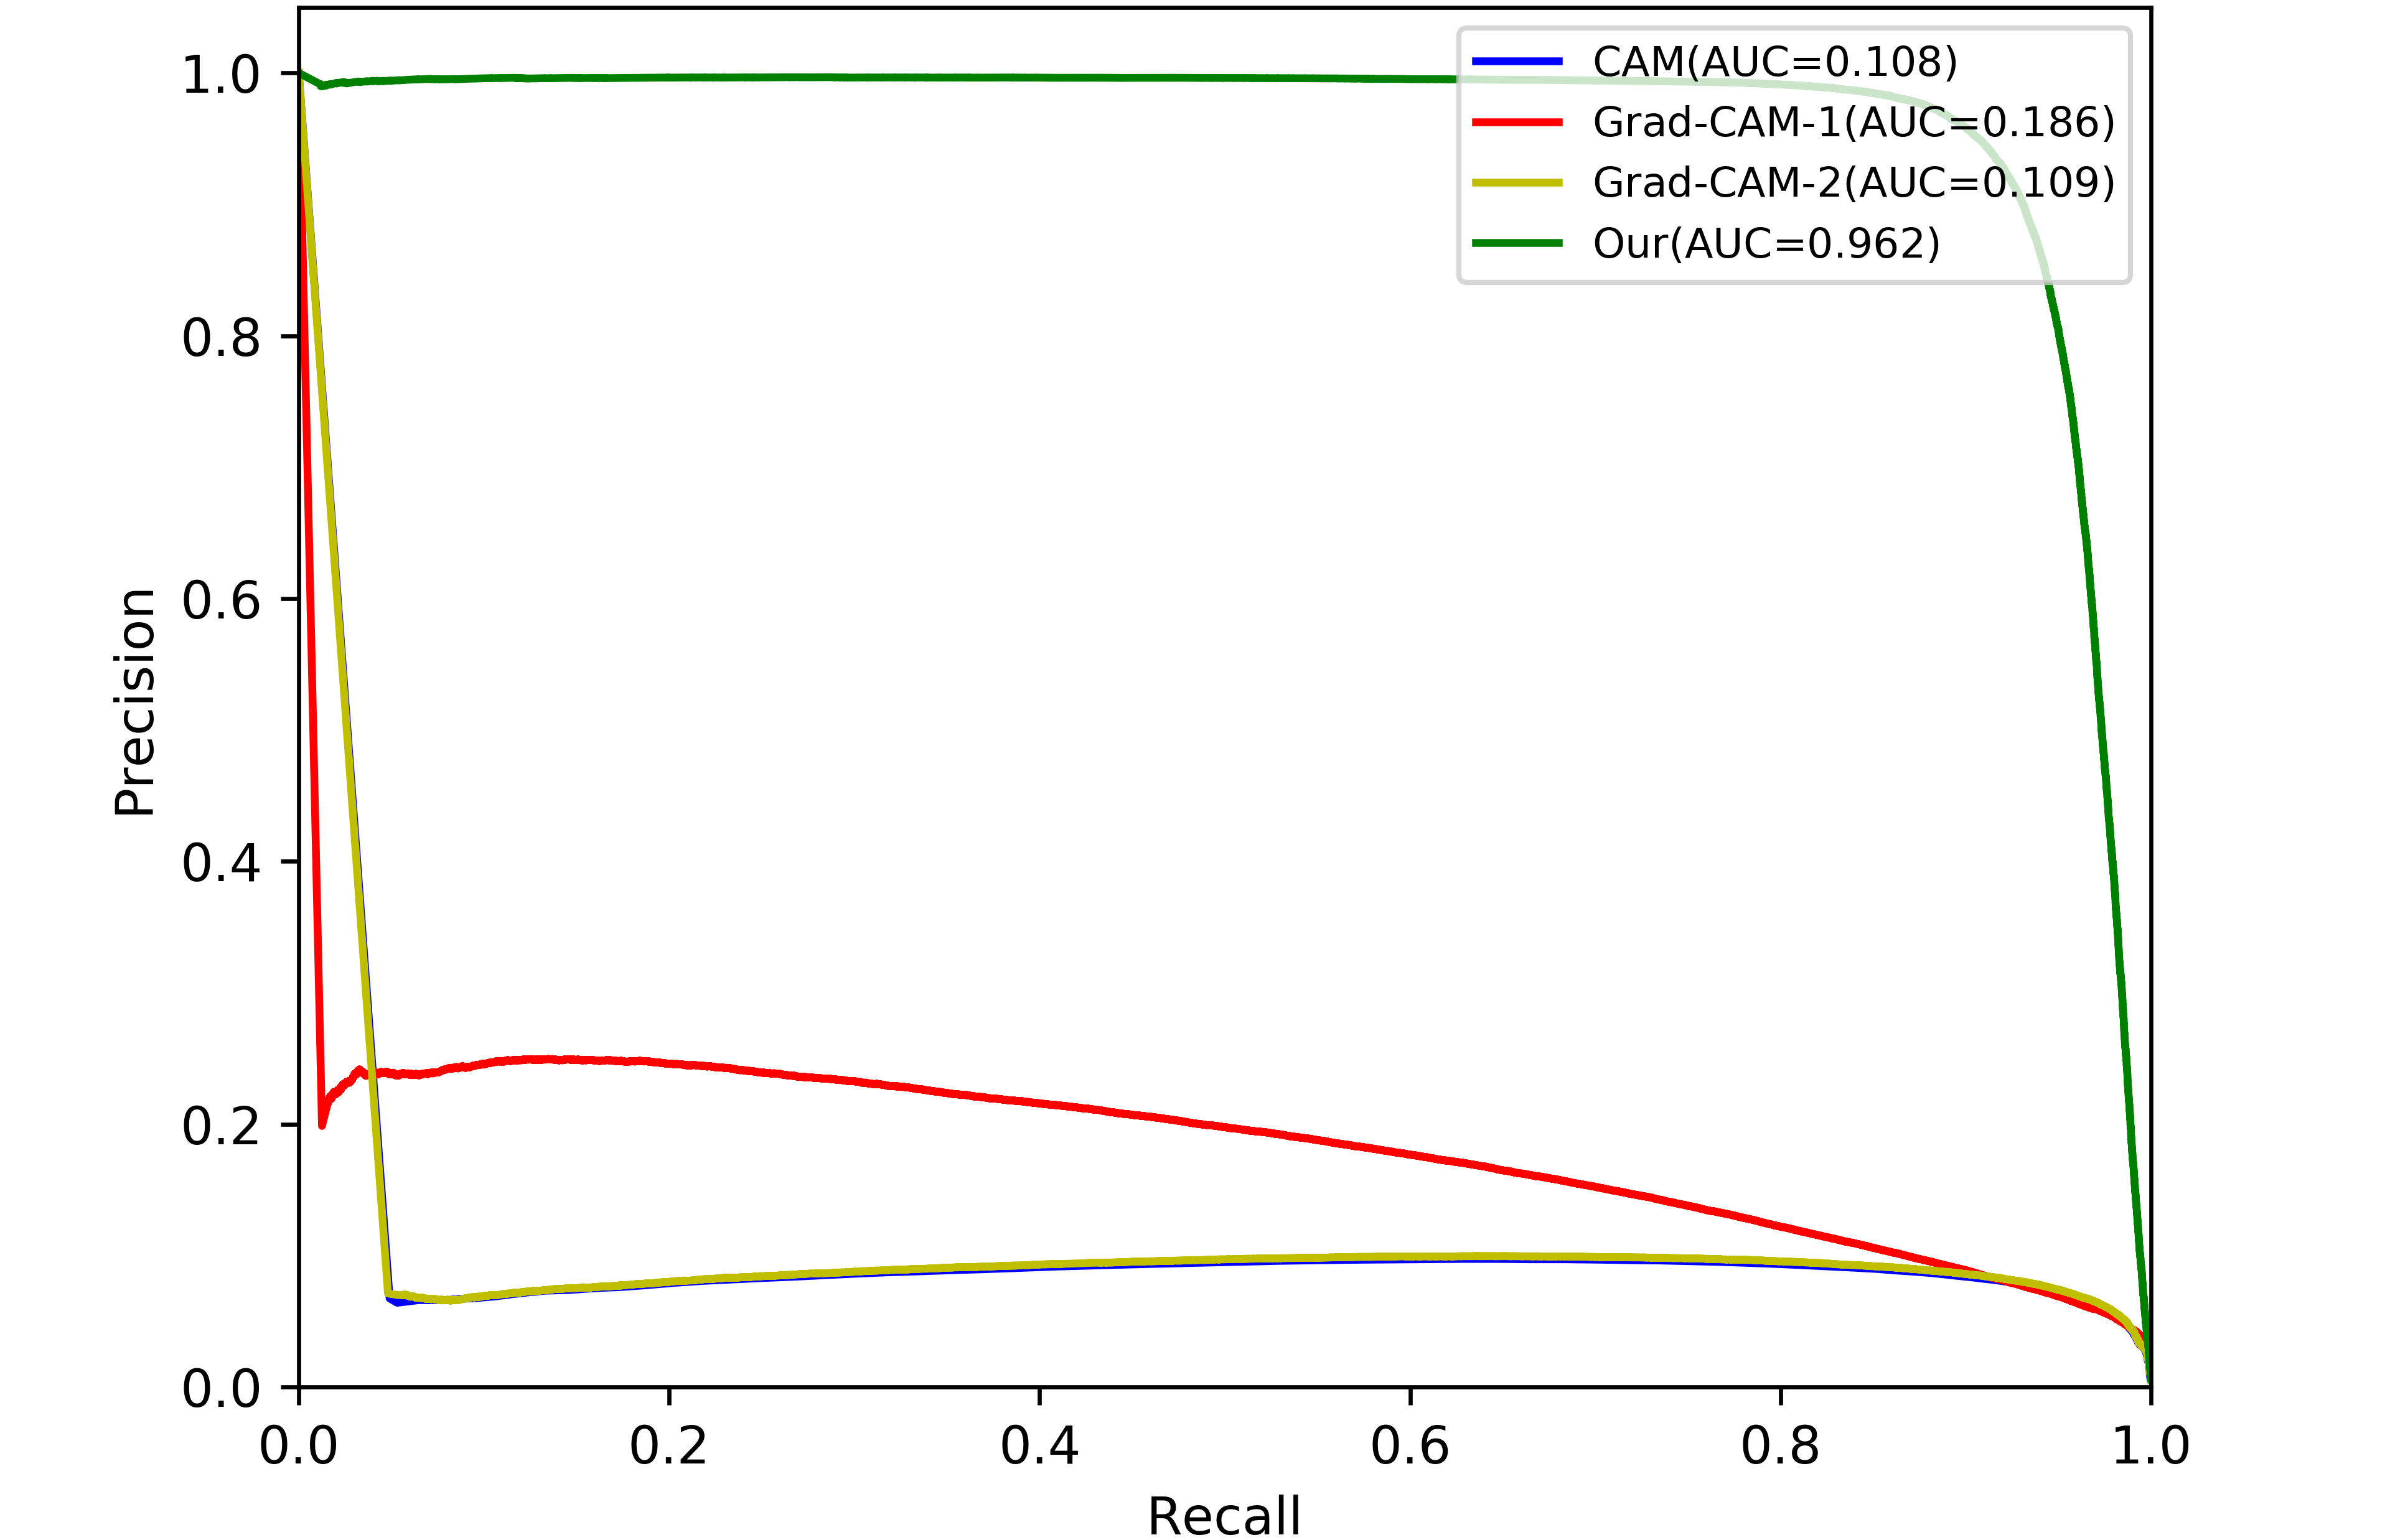
\includegraphics[width=0.6\textwidth]{figure/pr_curve_multi_skin/SKIN_pr_curve.png}
	\caption[第二类异常图像上P-R曲线对比]{第二类异常图像上P-R曲线对比。} 
	\label{fig:multi_simulate_pr_curve_skin}
\end{figure}
\begin{figure}[H]
	\centering
	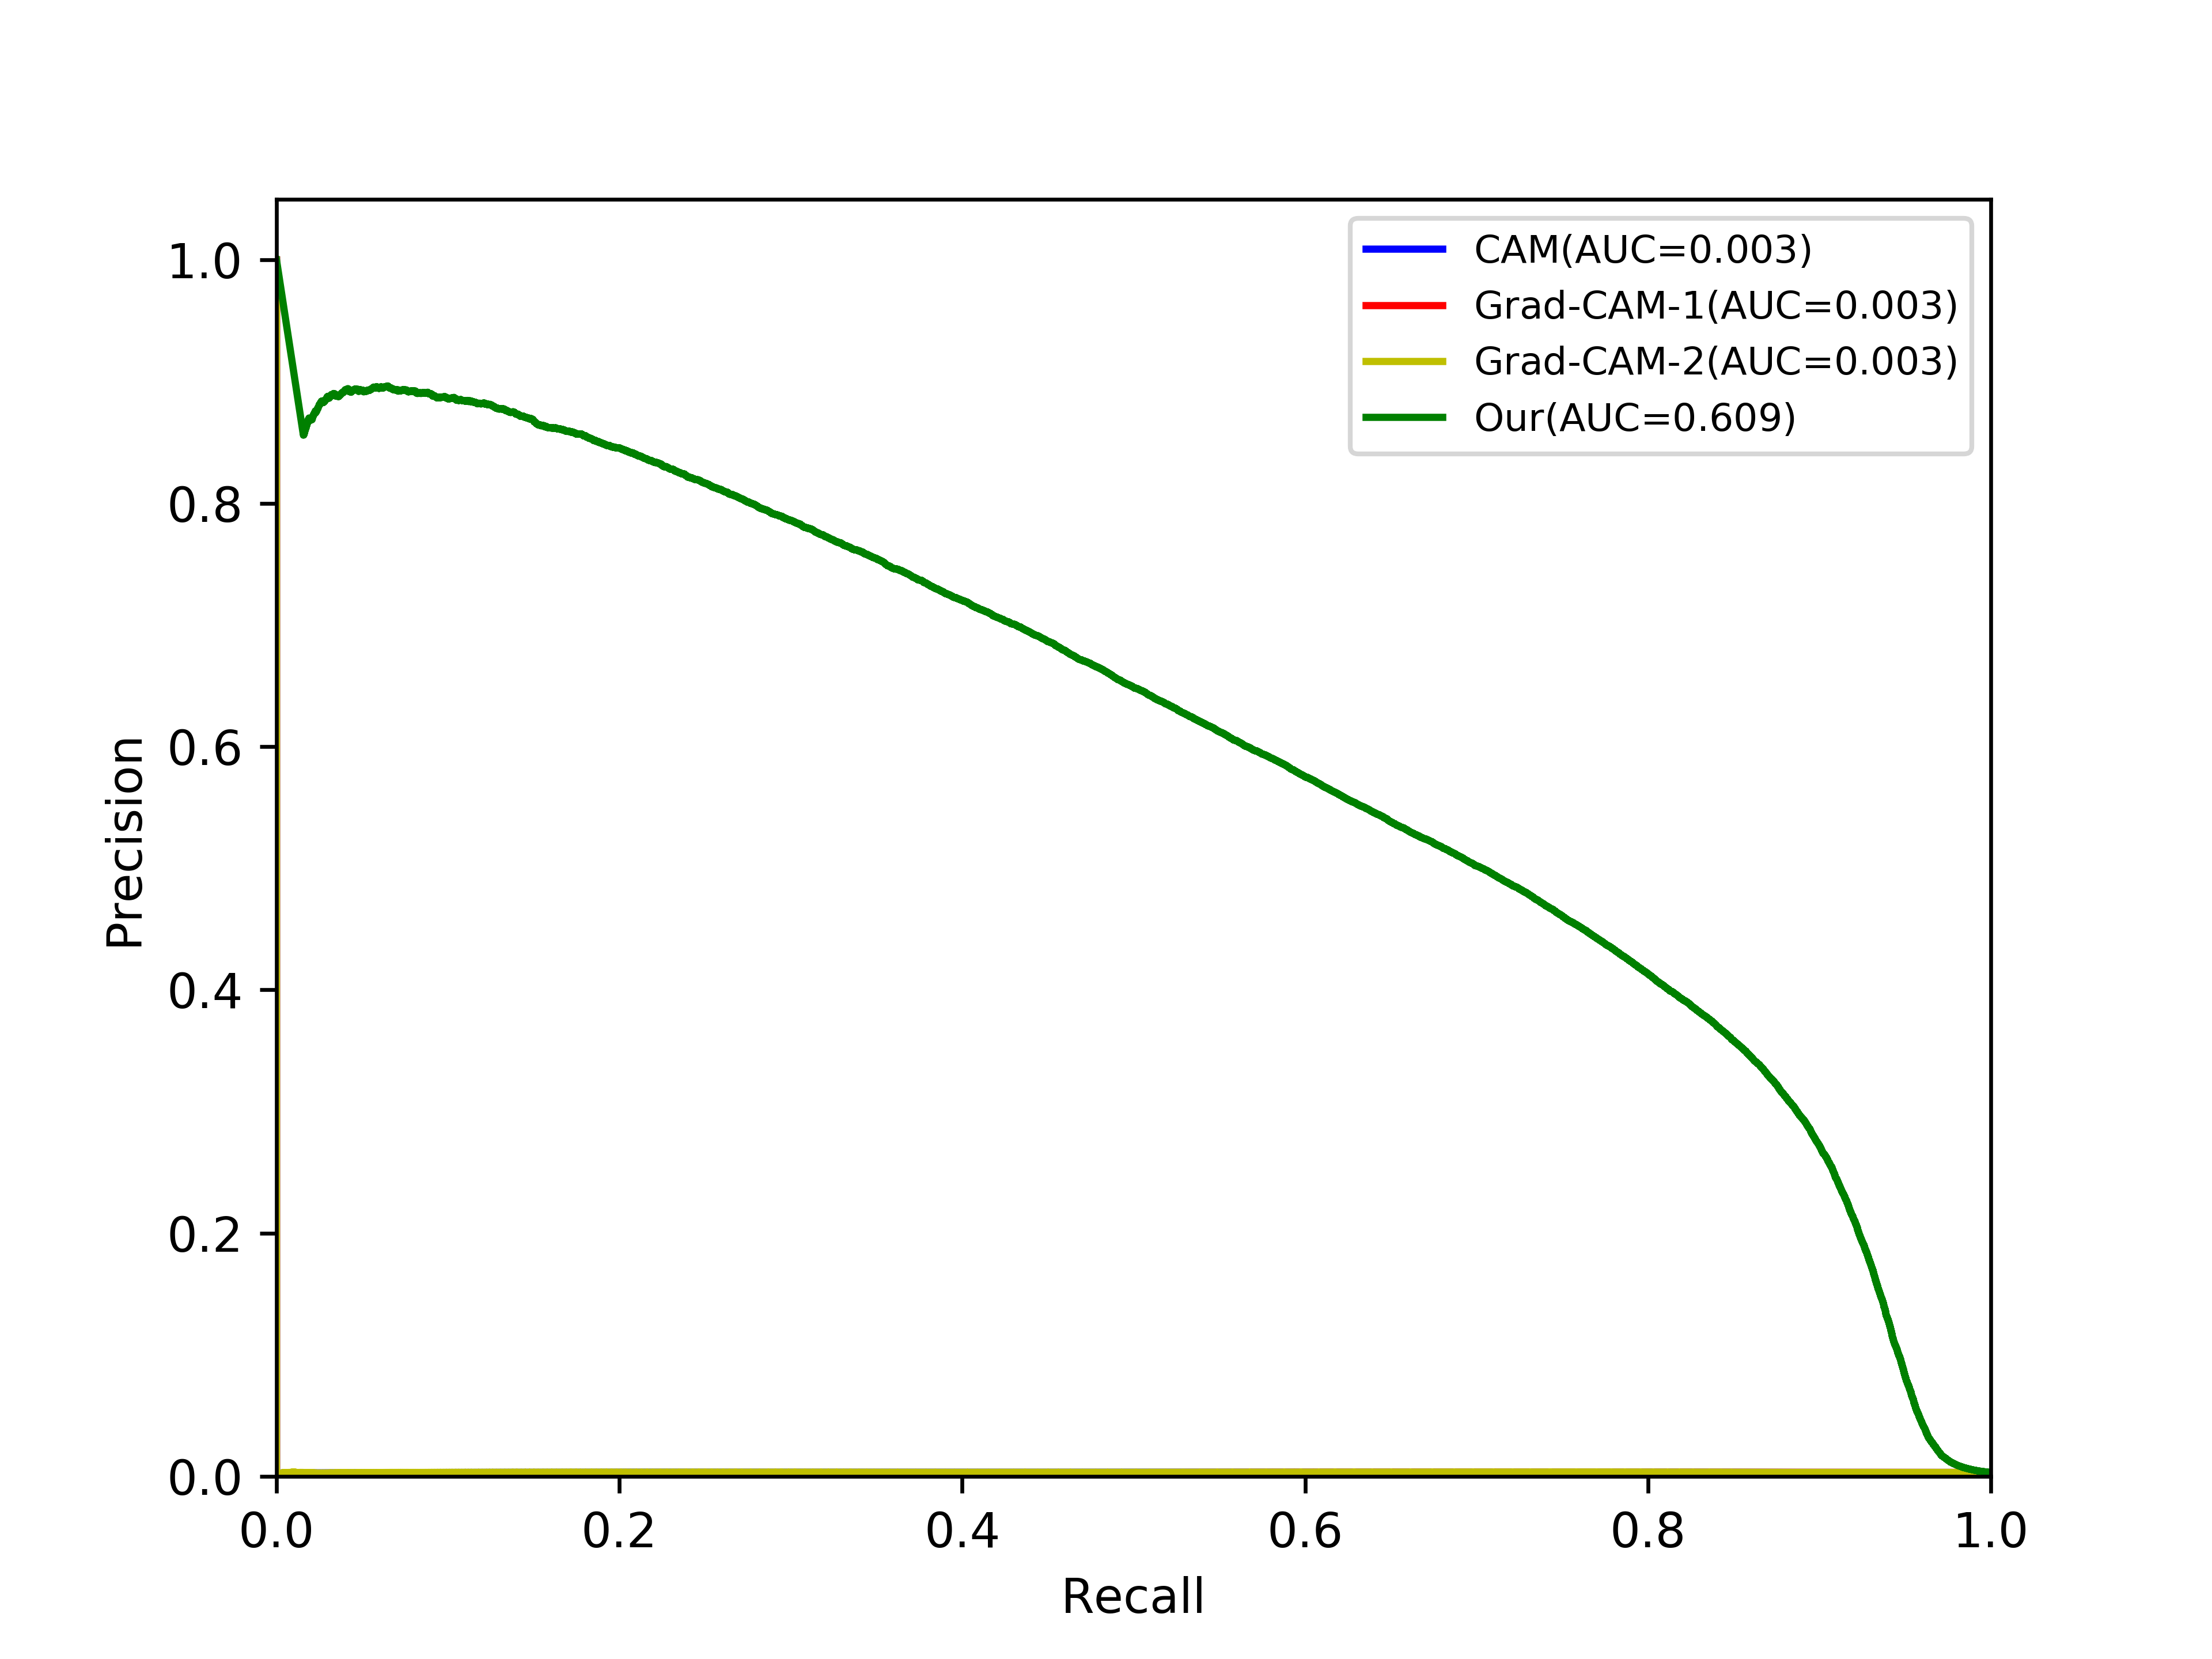
\includegraphics[width=0.6\textwidth]{figure/pr_curve_multi_skin/CIRCLE_pr_curve.png}
	\caption[第三类异常图像上P-R曲线对比]{第三类异常图像上P-R曲线对比。}
	\label{fig:multi_simulate_pr_curve_circle}
\end{figure}

如图\ref{fig:multi_simulate_pr_curve_image_net}所示,相比于其他两条曲线,绿色P-R曲线在其他三条曲线的上方,其AUC分数也最大(AUC=$0.236$),这说明了本文提出的方法相比于CAM和Grad-CAM能够更好地定位第一类异常图像中的疾病标记物。根据图\ref{fig:multi_simulate_pr_curve_skin}和图\ref{fig:multi_simulate_pr_curve_circle},我们也可以得出相同的结论,绿色曲线的AUC分数也都高于其他两条曲线,图\ref{fig:multi_simulate_pr_curve_skin}和图\ref{fig:multi_simulate_pr_curve_circle}中绿色P-R曲线的AUC分数分别为$0.962$和$0.805$,这远远大于图中其他三条P-R曲线的AUC分数,这说明相比于CAM和Grad-CAM,本文提出的方法在定位第二类异常和第三类异常对应的疾病标记物任务上同样有更好的性能。在表\ref{tab:multi_ds_auc_scores}中,本文提出的方法在三类异常图像上的平均AUC为$0.668$,远远高于CAM和Grad-CAM,这更直观地说明了上述结论。

总之,以上实验结果分别从定性分析和定量分析角度说明了,对于多类疾病标记物定位问题,即使疾病标记物在异常图像中分布广泛、大小各异,本文提出的方法相比于CAM和Grad-CAM仍然能够更精确地定位疾病标记物。
\begin{table}[!htbp]
	\centering
	\caption[三种疾病标记物定位方法在三类异常图像上的平均AUC分数]{本文提出的方法、CAM、Grad-CAM-1和Grad-CAM-2在三类异常图像上的平均AUC分数。}
	\label{tab:multi_ds_auc_scores}
	\begin{tabular}{c|c|c|c|c}
		\toprule[2pt]
		方法 & CAM & Grad-CAM-1 & Grad-CAM-2 & 本文提出的方法 \\
		\midrule[2pt]
%		第一类异常&$0.098$ & $0.224$ &  $0.098$ & $\textbf{0.236}$ \\ \hline
%		第二类异常&  $0.108$ &$0.186$ & $0.109$ & $\textbf{0.962}$ \\ \hline
%		第三类异常 & $0.003$ & $0.003$ & $0.003$ & $\textbf{0.805}$ \\ \hline
		Average AUC & $0.070$ & $0.138$ & $0.070$ & $\textbf{0.668}$ \\
		\bottomrule[2pt]
	\end{tabular}
\end{table}
\vspace{-0.7cm}
\section{对于经过编码器-解码器的多类模拟皮肤病病变图像的定量分析}
在本节中,本文同样将设置一组实验从间接角度证明本文提出的模型能够较好去除异常图像中的疾病标记物。与\ref{sec:indirect_quantitative_evaluation}小节中的设计思想相同,在理想情况下,如果一种方法能够完全去除疾病标记物,则去除疾病标记物之后的图像将不再包含疾病标记物,则这些图像很难与正常图像分开。根据以上前提假设,我们将多类模拟皮肤病病变数据集按照$80\%$和$20\%$的比例分为训练集和验证集(下文简称为“原始四类数据集”),随后用训练集训练一个ResNet-18四分类器。接着,我们将原始四类数据集中的每一张图像作为输入送入编码器-解码器,并将输出收集起来,这样我们得到一个新的数据集(下文简称为“‘正常’四类数据集”)。最后,我们用上述ResNet-18对“正常”四类数据集中的每一张图像进行分类。与\ref{sec:indirect_quantitative_evaluation}小节不同的是,我们不选定Recall和Specificity作为评价标准,这是因为多类问题中异常图像作为输入经过编码器-解码器之后的输出可能会向其他异常类转变而二类问题中异常图像作为输入经过编码器-解码器之后的输出只能向正常图像转变。因此,编码器-解码器对于正常图像输入的保持能力可定义为:
\begin{equation}\label{equ:normal_imgs_kep_rate}
\text{正常类的转化率}=\frac{\text{输出正常图像中被判定为异常的图像数量}}{\text{输入正常图像的数量}}.
\end{equation}

\noindent 同理,编码器-解码器对于异常图像输入的转化能力可定义为:

\begin{equation}\label{equ:lesion_imgs_converted_rate}
\text{异常类的转化率}=\frac{\text{输出异常图像中被判定为正常的图像数量}}{\text{输入异常图像的数量}}.
\end{equation}

\noindent 显然,正常类的转化率越低而异常类的转化率越高表示模型定位并去除疾病标记物的能力越强。基于以上设置得到的实验结果如表\ref{tab:quantitative_simulated_skin}所示,前两列表示在原始四类数据集上的实验结果,后两列表示“正常”四类数据集上的实验结果。

\begin{table}[h!]
	\centering
	\caption[ResNet-18四分类器对原始四类数据集和“正常”四类数据集的分类结果]{ResNet-18四分类器对原始四类数据集和“正常”四类数据集的分类结果。} 
	\label{tab:quantitative_simulated_skin}
	\begin{tabular}{c|cc|cc}
		\toprule[2pt]
		& \multicolumn{2}{c|}{\shortstack{原始四类数据集\\\scriptsize{(分类正确率)}}} &\multicolumn{2}{c}{\shortstack{“正常”四类数据集\\\scriptsize{(转化率)}}} \\
		&  训练集 & 验证集 & 训练集 & 验证集\\
		\midrule[2pt]
		正常类 & $0.992$ & $0.989$ & $0.094$ & $0.097$\\ \hline
		第一类异常 & $0.985$ & $0.981$ & $0.753$ & $0.741$\\ \hline
		第二类异常 & $0.999$ & $0.986$ & $0.976$ & $0.981$\\ \hline
		第三类异常 & $1.000$ & $1.000$ & $0.856$ & $0.840$\\
		\bottomrule[2pt]
	\end{tabular}
\end{table}

我们可以从表\ref{tab:quantitative_simulated_skin}中前两列看出,对于原始四类数据集,无论是正常类还是三个异常类,训练集和验证集上分类正确率均达到了$98\%$以上,这表明ResNet-18四类分类器可以很好学习到疾病标记物的相关特征。而在该表的后两列中,我们可以发现,对于“正常”四类数据集中的三个异常类,异常图像的转化率都比较高,尤其是第二类异常,训练集和验证集上的转化率分别达到了$97.6\%$和$98.1\%$,以上结果可表明编码器-解码器对于异常图像输入有较好的转化能力,可以很好的定位并去除疾病标记物。相比之下,正常类的转化率要低得多,在训练集和验证集上的转化率分别为$9.4\%$和$9.7\%$,这可以说明编码器-解码器对于正常图像输入有较好的保持能力。
\begin{figure}[h]
	\centering
	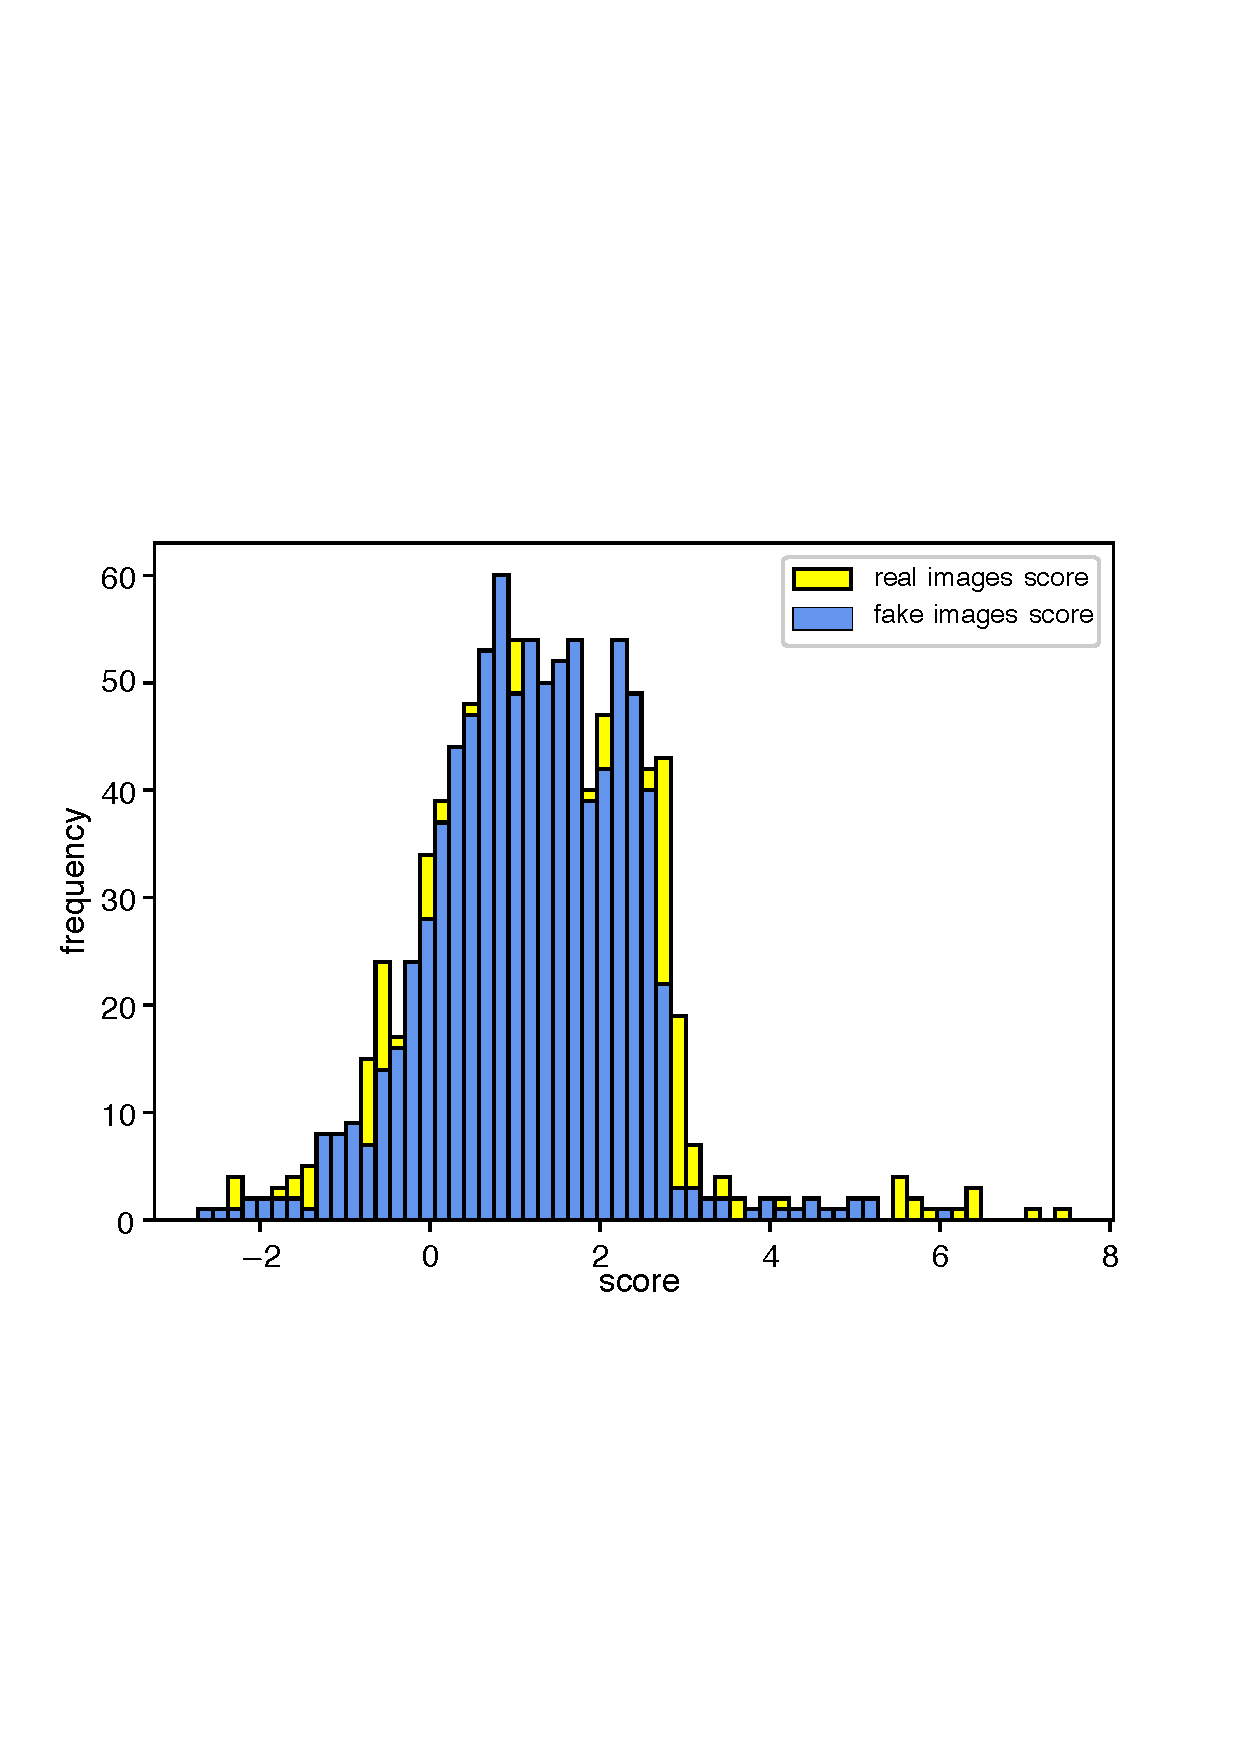
\includegraphics[width=0.9\textwidth]{figure/simulated_skin_score_distribution.pdf}
	\caption[判别器输出分数频率分布直方图]{判别器输出分数频率分布直方图。多类模拟皮肤病变数据集中的正常图像(真图像)和该数据集中的异常图像经过编码器-解码器的输出图像(假图像)作为判别器输入。}
	\label{fig:simulated_skin_hist_freq}
\end{figure}

以上实验从额外训练的ResNet分类器间接说明了本文提出的模型能很好地去除疾病标记物。在本小节中,我们还将多类模拟皮肤病病变数据集中的正常图像(以下简称“真图像”)和多类模拟皮肤病病变数据集中的异常图像经过编码器-解码器的输出图像(以下简称“假图像”)分别送入判别器,判别器输出分数的频率分布直方图如图\ref{fig:simulated_skin_hist_freq}所示,图中黄色柱子表示判别器对真图像的输出分数,蓝色柱子表示判别器对假图像的输出分数。从图\ref{fig:simulated_skin_hist_freq}中我们可以发现蓝色柱子和黄色柱子有较大重叠面积。我们计算得到判别器对真图像和假图像的平均输出分数分别为$1.3 $和$1.2$。而在初始参数下,两者分别为$2.5$和$-0.5$,这说明在训练结束后,真图像和假图像的相似性得到了极大提升(平均分数差距显著缩小:$3.0\rightarrow 0.1$),异常图像经过编码器-解码器的输出图像已经十分接近正常图像,由此可以推断出编码器-解码器已经很好地去除了异常图像中的疾病标记物。

总之,通过对经过编码器-解码器的多类模拟皮肤病病变图像的定量分析,本小节分别从额外训练的分类器角度和本文提出的模型本身的判别器角度间接说明了本文提出的方法能够比较好地去除异常图像中的疾病标记物。
\section{不同超参数下的实验结果分析}\label{sec:multi_classes_hyper_paras}
在本小节中,本文继续探究在不同超参数$\lambda_{1}$和$\lambda_{2}$组合下,本文提出的模型在疾病标记物定位任务上的性能表现,以评估本文提出的模型的鲁棒性。在学习率、优化器、迭代次数、模型结构等设置均保持不变的情况下,除了默认超参数组合外($\lambda_{1}=4.0,\lambda_{2}=20.0$),我们还选取了另外$6$组不同超参数。在多类模拟皮肤病病变数据集上完成了相关实验后,分别根据第一类异常、第二类异常和第三类异常图像所绘制的P-R曲线分别如图\ref{fig:multi_simulate_pr_curve_image_net_hyper_paras}、图\ref{fig:multi_simulate_pr_curve_skin_hyper_paras}和图\ref{fig:multi_simulate_pr_curve_circle_hyper_paras}所示。为了更直观地比较不同超参数下的模型性能,我们将以上P-R曲线在三个异常类上的平均AUC分数列在表\ref{tab:simulated_skin_diff_parameters}中。

从图\ref{fig:multi_simulate_pr_curve_image_net_hyper_paras}和图\ref{fig:multi_simulate_pr_curve_skin_hyper_paras}可以看出,绿色P-R曲线明显在其他曲线上方,这说明本文提出的模型在默认参数($\lambda_{1}=4,\lambda_{2}=20$)下,定位第一类异常和第二类异常对应的疾病标记物的性能最佳。相反,在图\ref{fig:multi_simulate_pr_curve_circle_hyper_paras}中,黄色P-R曲线($\lambda_{1}=10,\lambda_{2}=20$)的AUC最大(AUC为$0.823$),这是因为第三类异常对应的疾病标记物相比第一类异常和第二类异常在图像中的数量更多、分布的范围也更广,因而交叉熵损失函数权重较大更有利于本文提出的模型更全面地定位到第三类异常对应的疾病标记物。从平均AUC分数来看(见表\ref{tab:simulated_skin_diff_parameters}),本文提出的模型在默认参数下平均AUC分数最高(AUC=$0.668$,表中第一列)。相比于默认参数(绿色P-R曲线),当超参数$\lambda_{1}$偏小甚至取$0$时,在图\ref{fig:multi_simulate_pr_curve_image_net_hyper_paras}和图\ref{fig:multi_simulate_pr_curve_skin_hyper_paras}和图\ref{fig:multi_simulate_pr_curve_circle_hyper_paras}中,深红色P-R曲线($\lambda_{1}=1$)和粉红色P-R曲线($\lambda_{1}=0$)的AUC分数均较低,尤其是图\ref{fig:multi_simulate_pr_curve_image_net_hyper_paras}中深红色P-R曲线的AUC最低(AUC=$0.135$)。这说明,一旦交叉熵损失函数在本文提出的模型中所占的权重($\lambda_{1}$)较小,本文提出的模型定位疾病标记物的性能也会有所下降,在极端情况($\lambda_{1}=0$)下,CNN分类器没有发挥任何作用,其AUC为$0.149$。当超参数$\lambda_{2}$偏小时,L1损失函数在本文提出的模型中所占权重较小,本文提出的模型对编码器-解码器的约束将会减弱,本文提出的模型在去除疾病标记物的同时也会不可避免地修改正常区域,比如青色P-R曲线($\lambda_{2}=10$)和黑色P-R曲线($\lambda_2=0$),在图\ref{fig:multi_simulate_pr_curve_image_net_hyper_paras}、图\ref{fig:multi_simulate_pr_curve_skin_hyper_paras}和图\ref{fig:multi_simulate_pr_curve_circle_hyper_paras}中这两条P-R曲线的AUC分数都较低,尤其是图\ref{fig:multi_simulate_pr_curve_image_net_hyper_paras}中青色P-R曲线,其AUC最低(AUC=$0.084$)。反之,当超参数$\lambda_{2}$偏大时,比如蓝色P-R曲线($\lambda_{2}=50$),通过图\ref{fig:multi_simulate_pr_curve_image_net_hyper_paras}、图\ref{fig:multi_simulate_pr_curve_skin_hyper_paras}和图\ref{fig:multi_simulate_pr_curve_circle_hyper_paras},我们均可以发现蓝色P-R曲线被绿色P-R曲线包围,更为直观的是看表\ref{tab:simulated_skin_diff_parameters}中的平均AUC分数,两者分别为$0.628$和$0.668$,这是因为当L1损失函数权重过大时限制了编码器-解码器对图像的修改,最终导致本文提出的模型定位异常图像中的疾病标记物的性能下降。根据表\ref{tab:simulated_skin_diff_parameters},我们可以发现第$2$列($\lambda_{1}=4,\lambda_{2}=20$)、第$4$列($\lambda_{1}=10,\lambda_{2}=20$)和$6$列($\lambda_{1}=4,\lambda_{2}=50$)的平均AUC较为接近,分别为$0.668$、$0.659$、$0.628$,这说明本文提出的模型的超参数适用范围较广,有较好鲁棒性。

综上,以上实验结果表明本文提出的方法具有较好鲁棒性,超参数$\lambda_{1}$和$\lambda_{2}$在极端情况下,本文提出的方法的定位性能有所下降,这也符合我们的预期。
\begin{figure}[H]
	\centering
	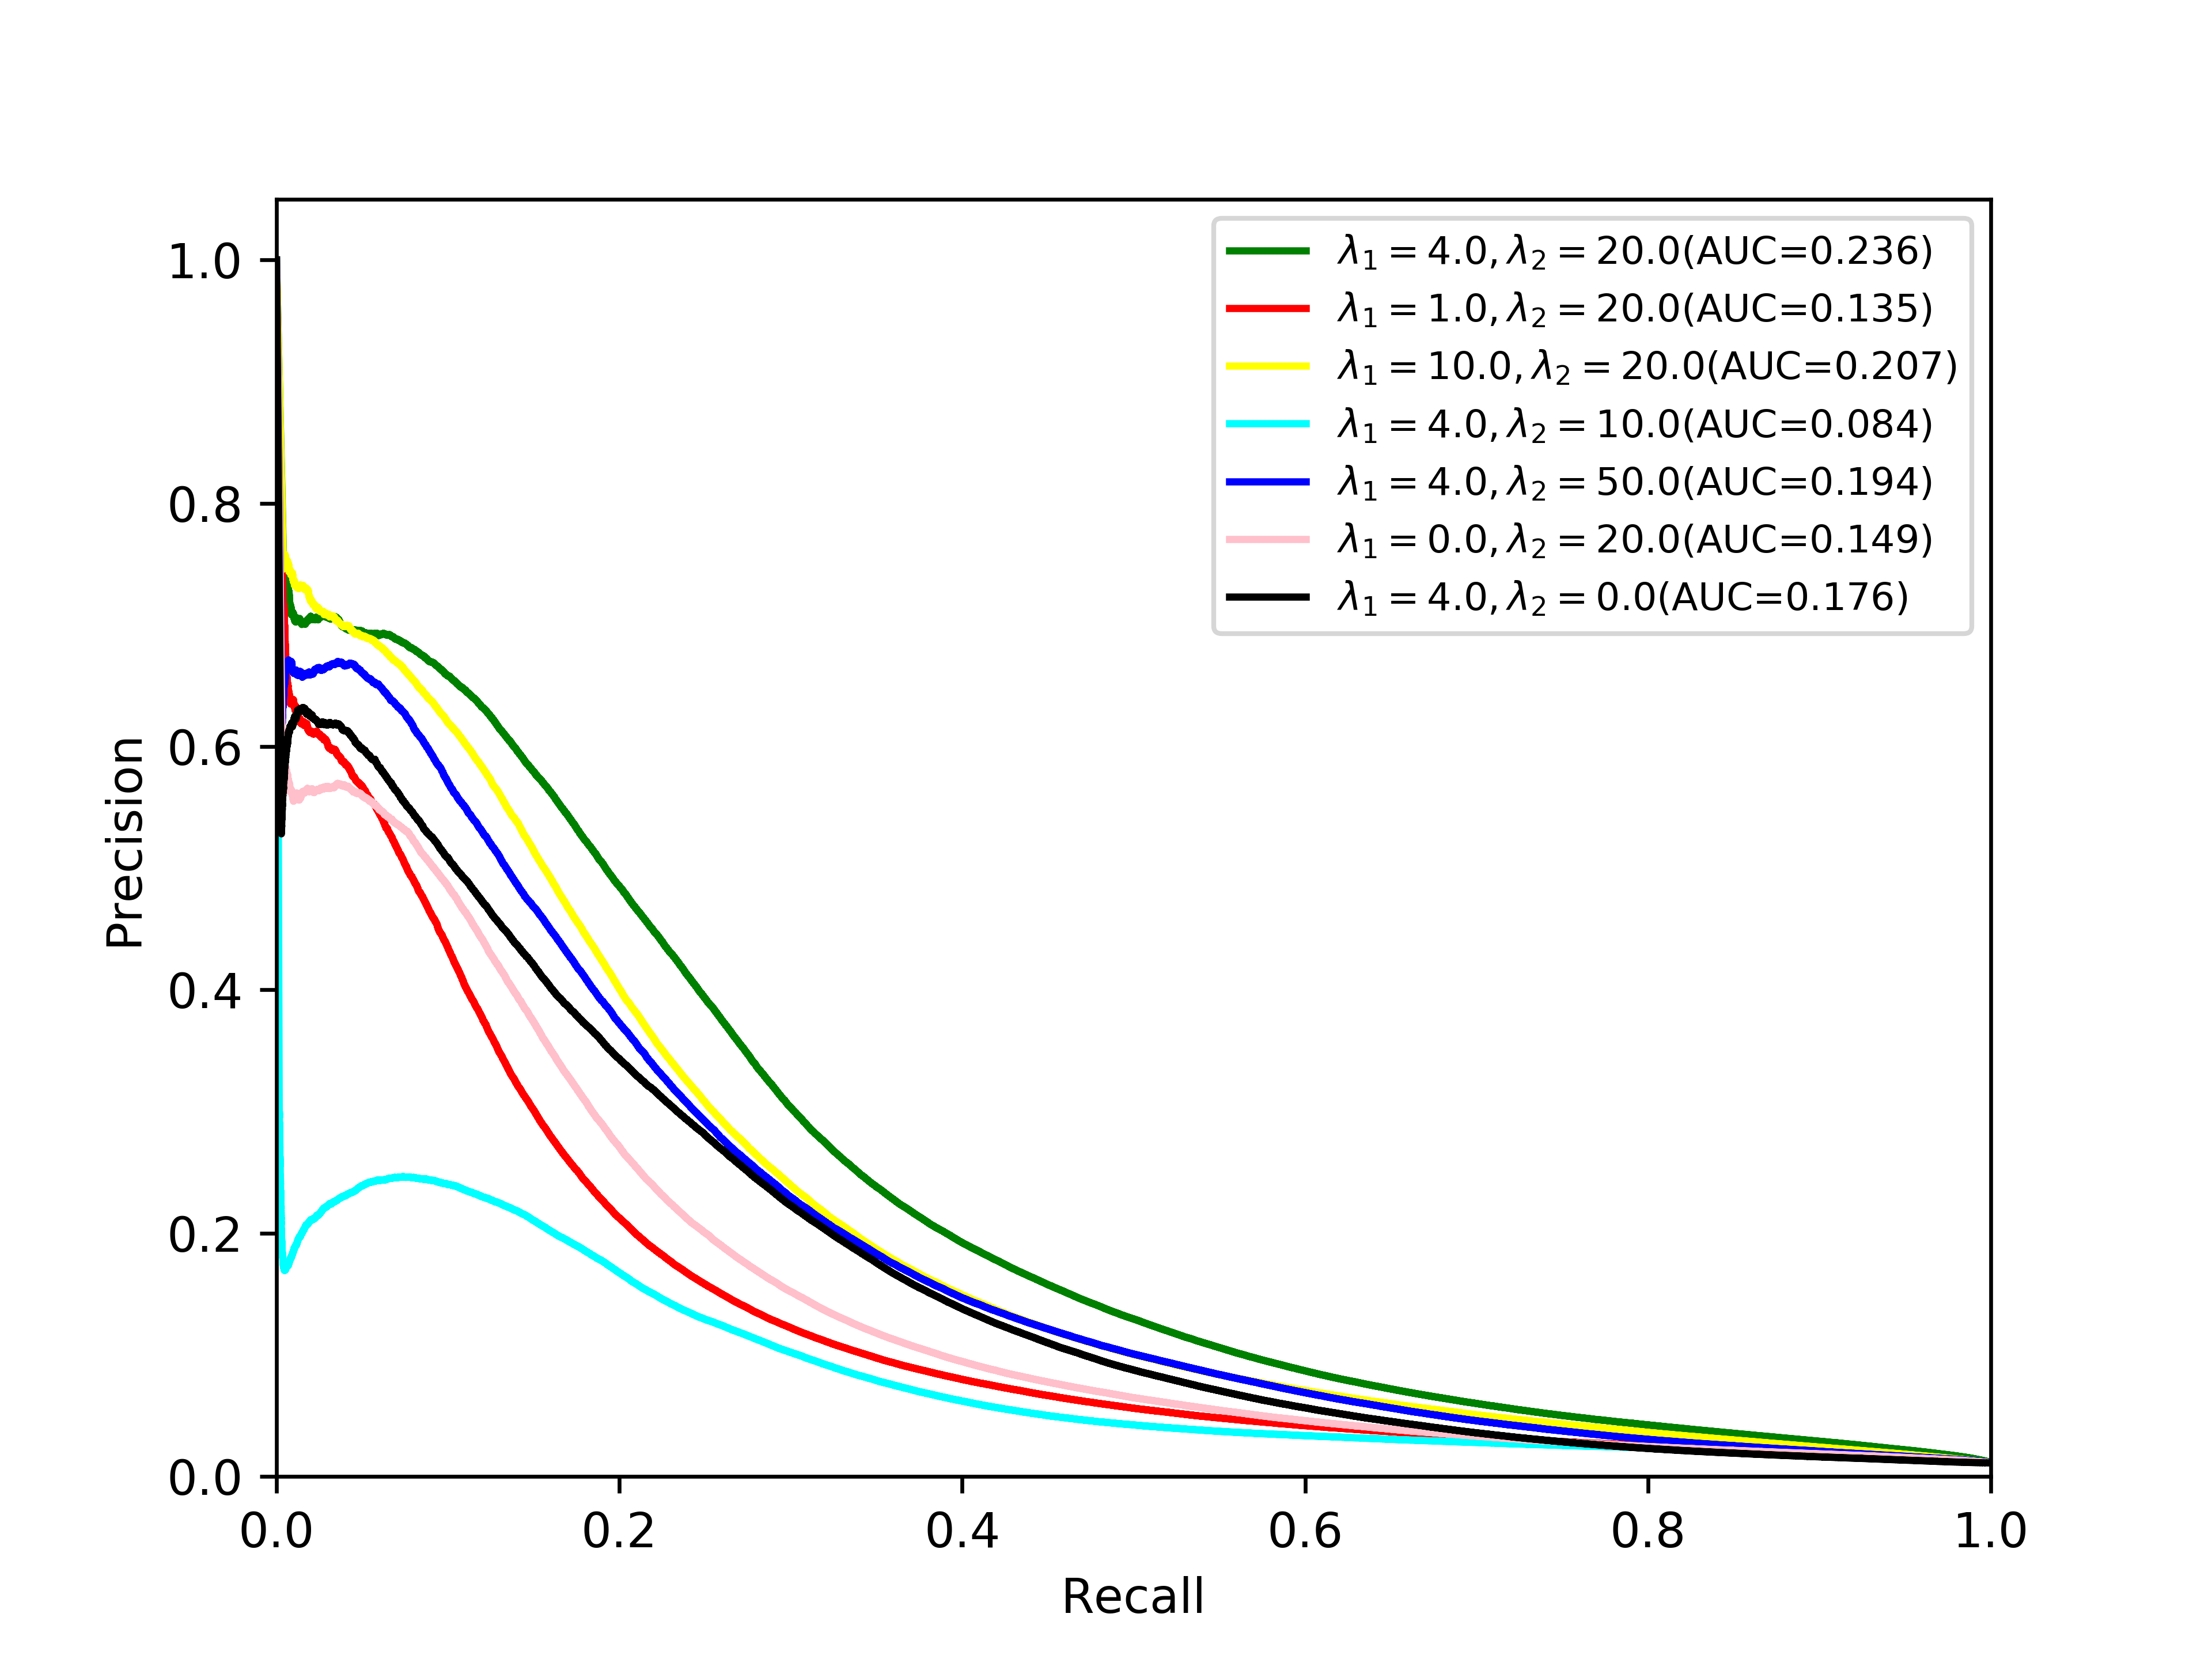
\includegraphics[width=0.6\textwidth]{figure/pr_curve_multi_skin_hyper_paras/IMAGE_NET_pr_curve.png}
	\caption[不同超参数组合下第一类异常图像上P-R曲线对比]{在多类模拟皮肤病病变数据集上,不同超参数组合下第一类异常图像上P-R曲线对比。} 
	\label{fig:multi_simulate_pr_curve_image_net_hyper_paras}
\end{figure}
\vspace{-0.3cm}
\begin{figure}[H]
	\centering
	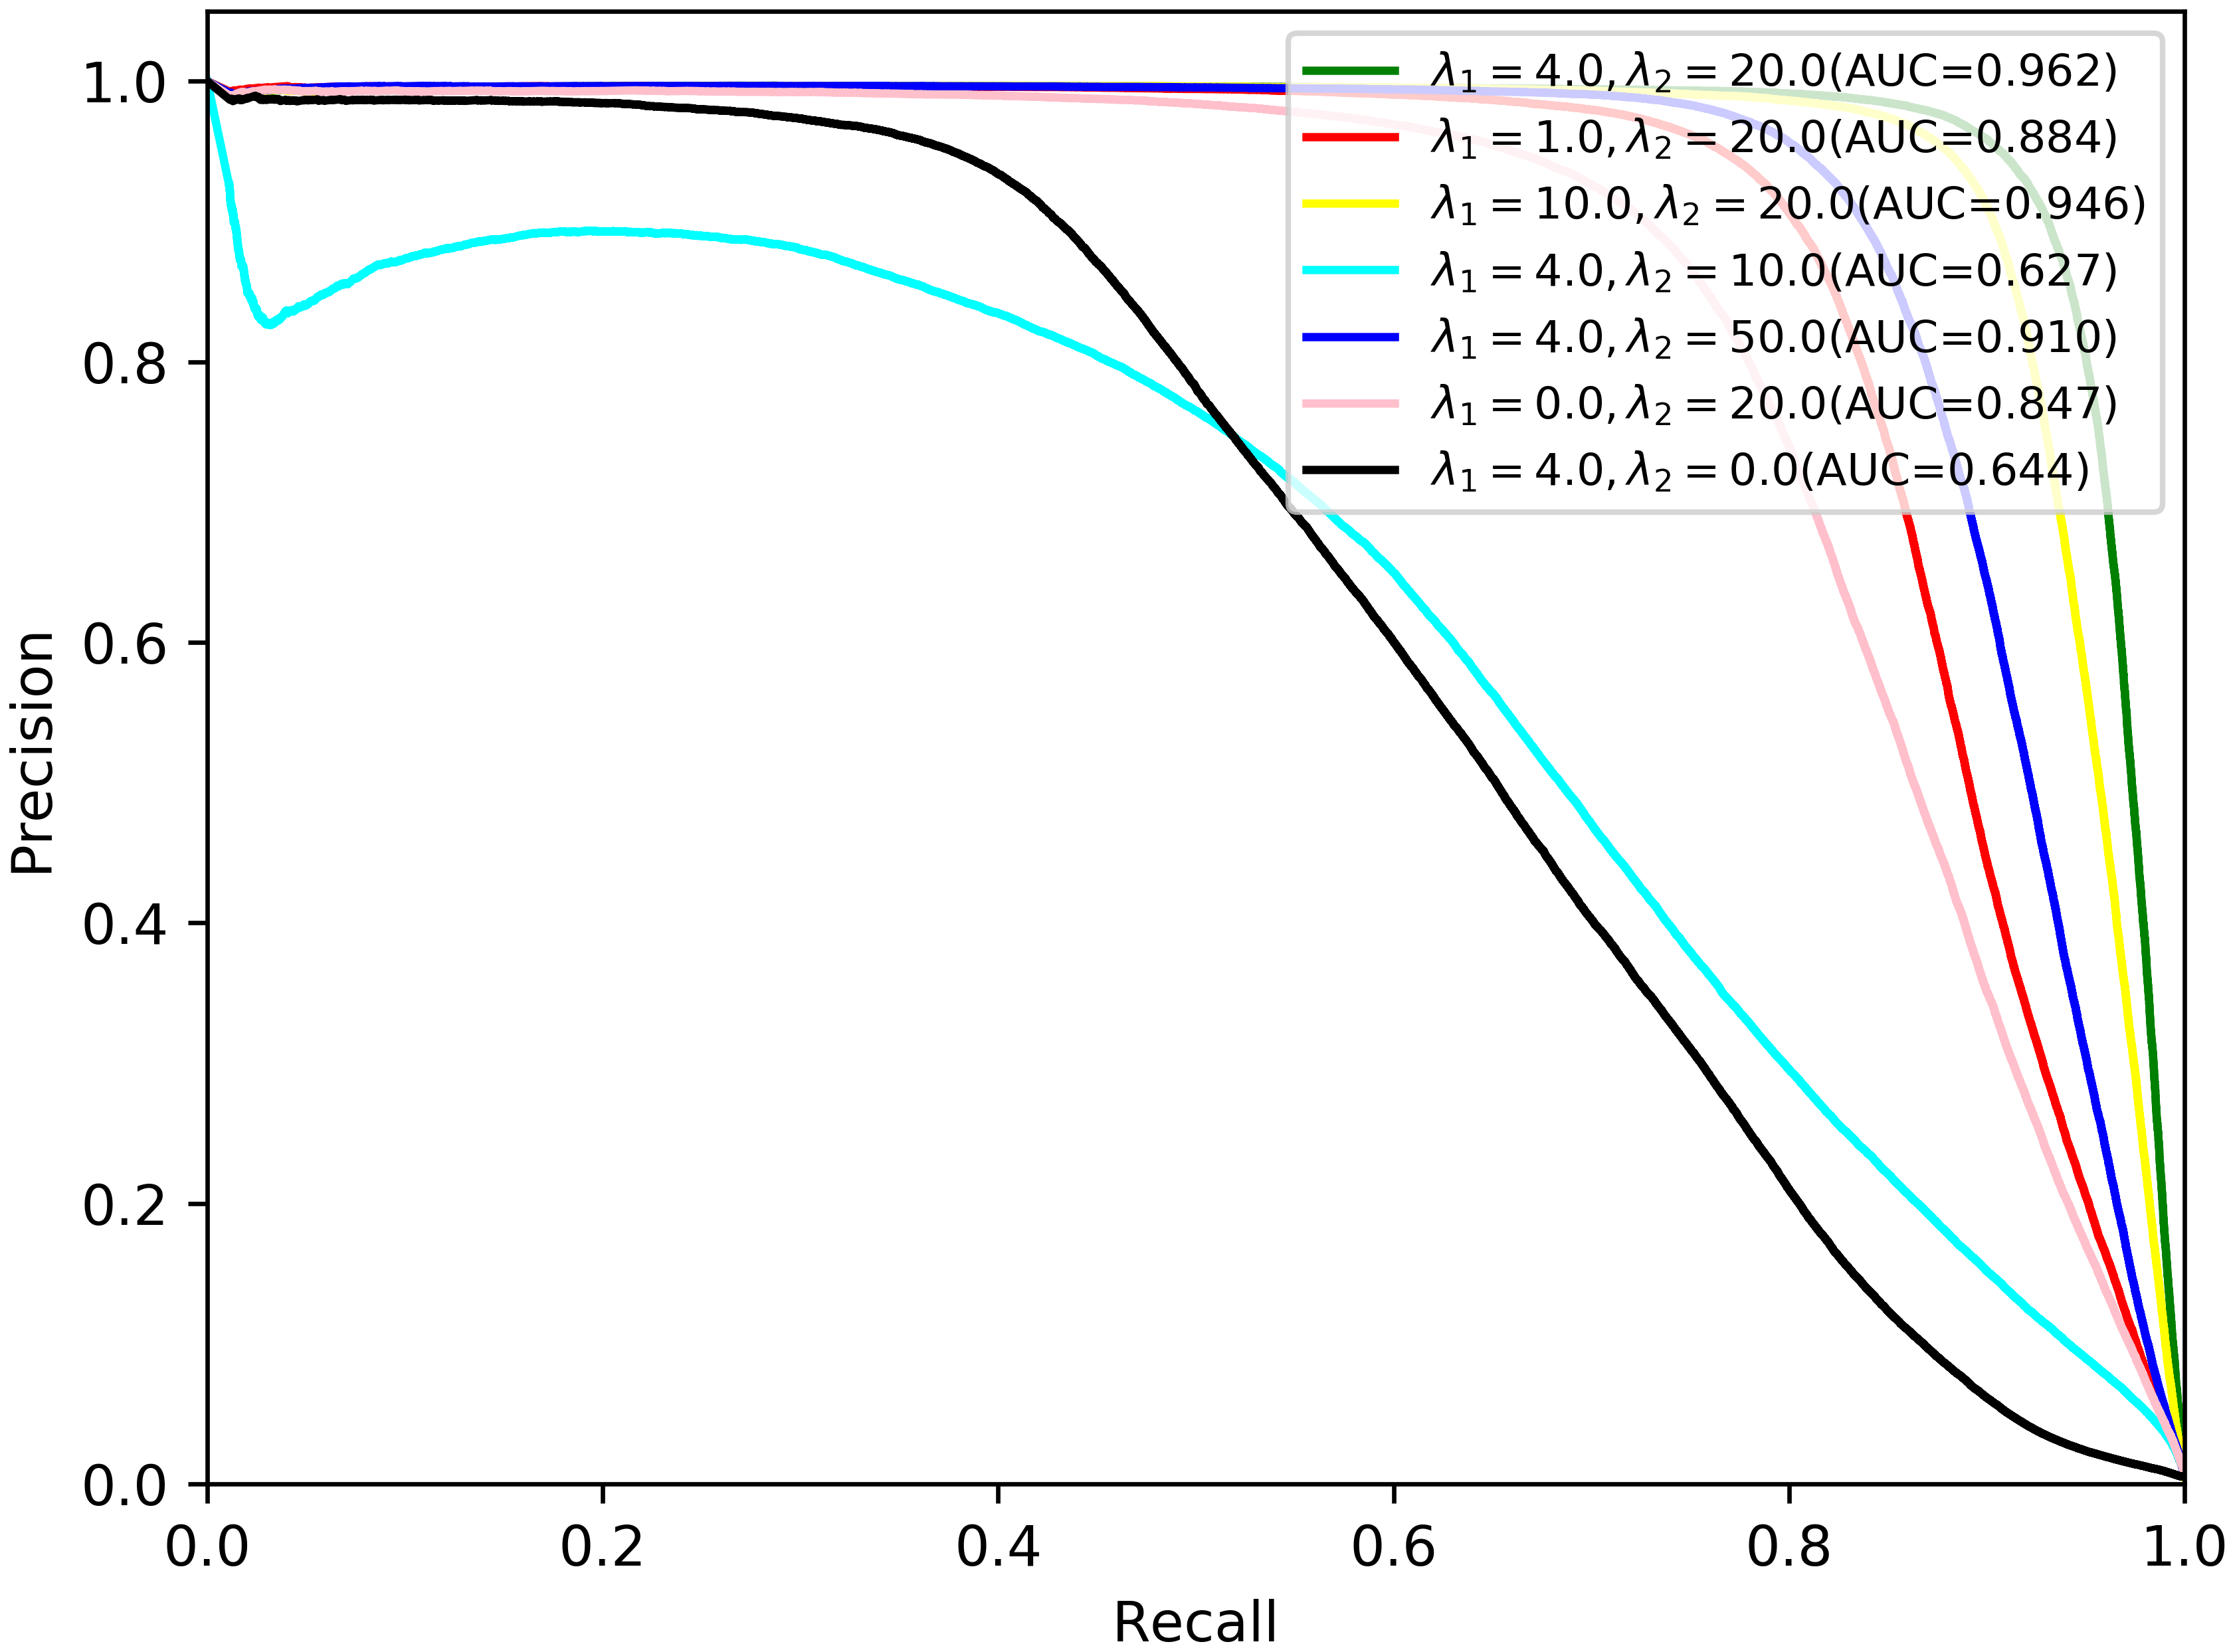
\includegraphics[width=0.6\textwidth]{figure/pr_curve_multi_skin_hyper_paras/SKIN_pr_curve.png}
	\caption[不同超参数组合下第二类异常图像上P-R曲线对比]{在多类模拟皮肤病病变数据集上,不同超参数组合下第二类异常图像上P-R曲线对比。}
	\label{fig:multi_simulate_pr_curve_skin_hyper_paras}
\end{figure}
\begin{figure}[H]
	\centering
	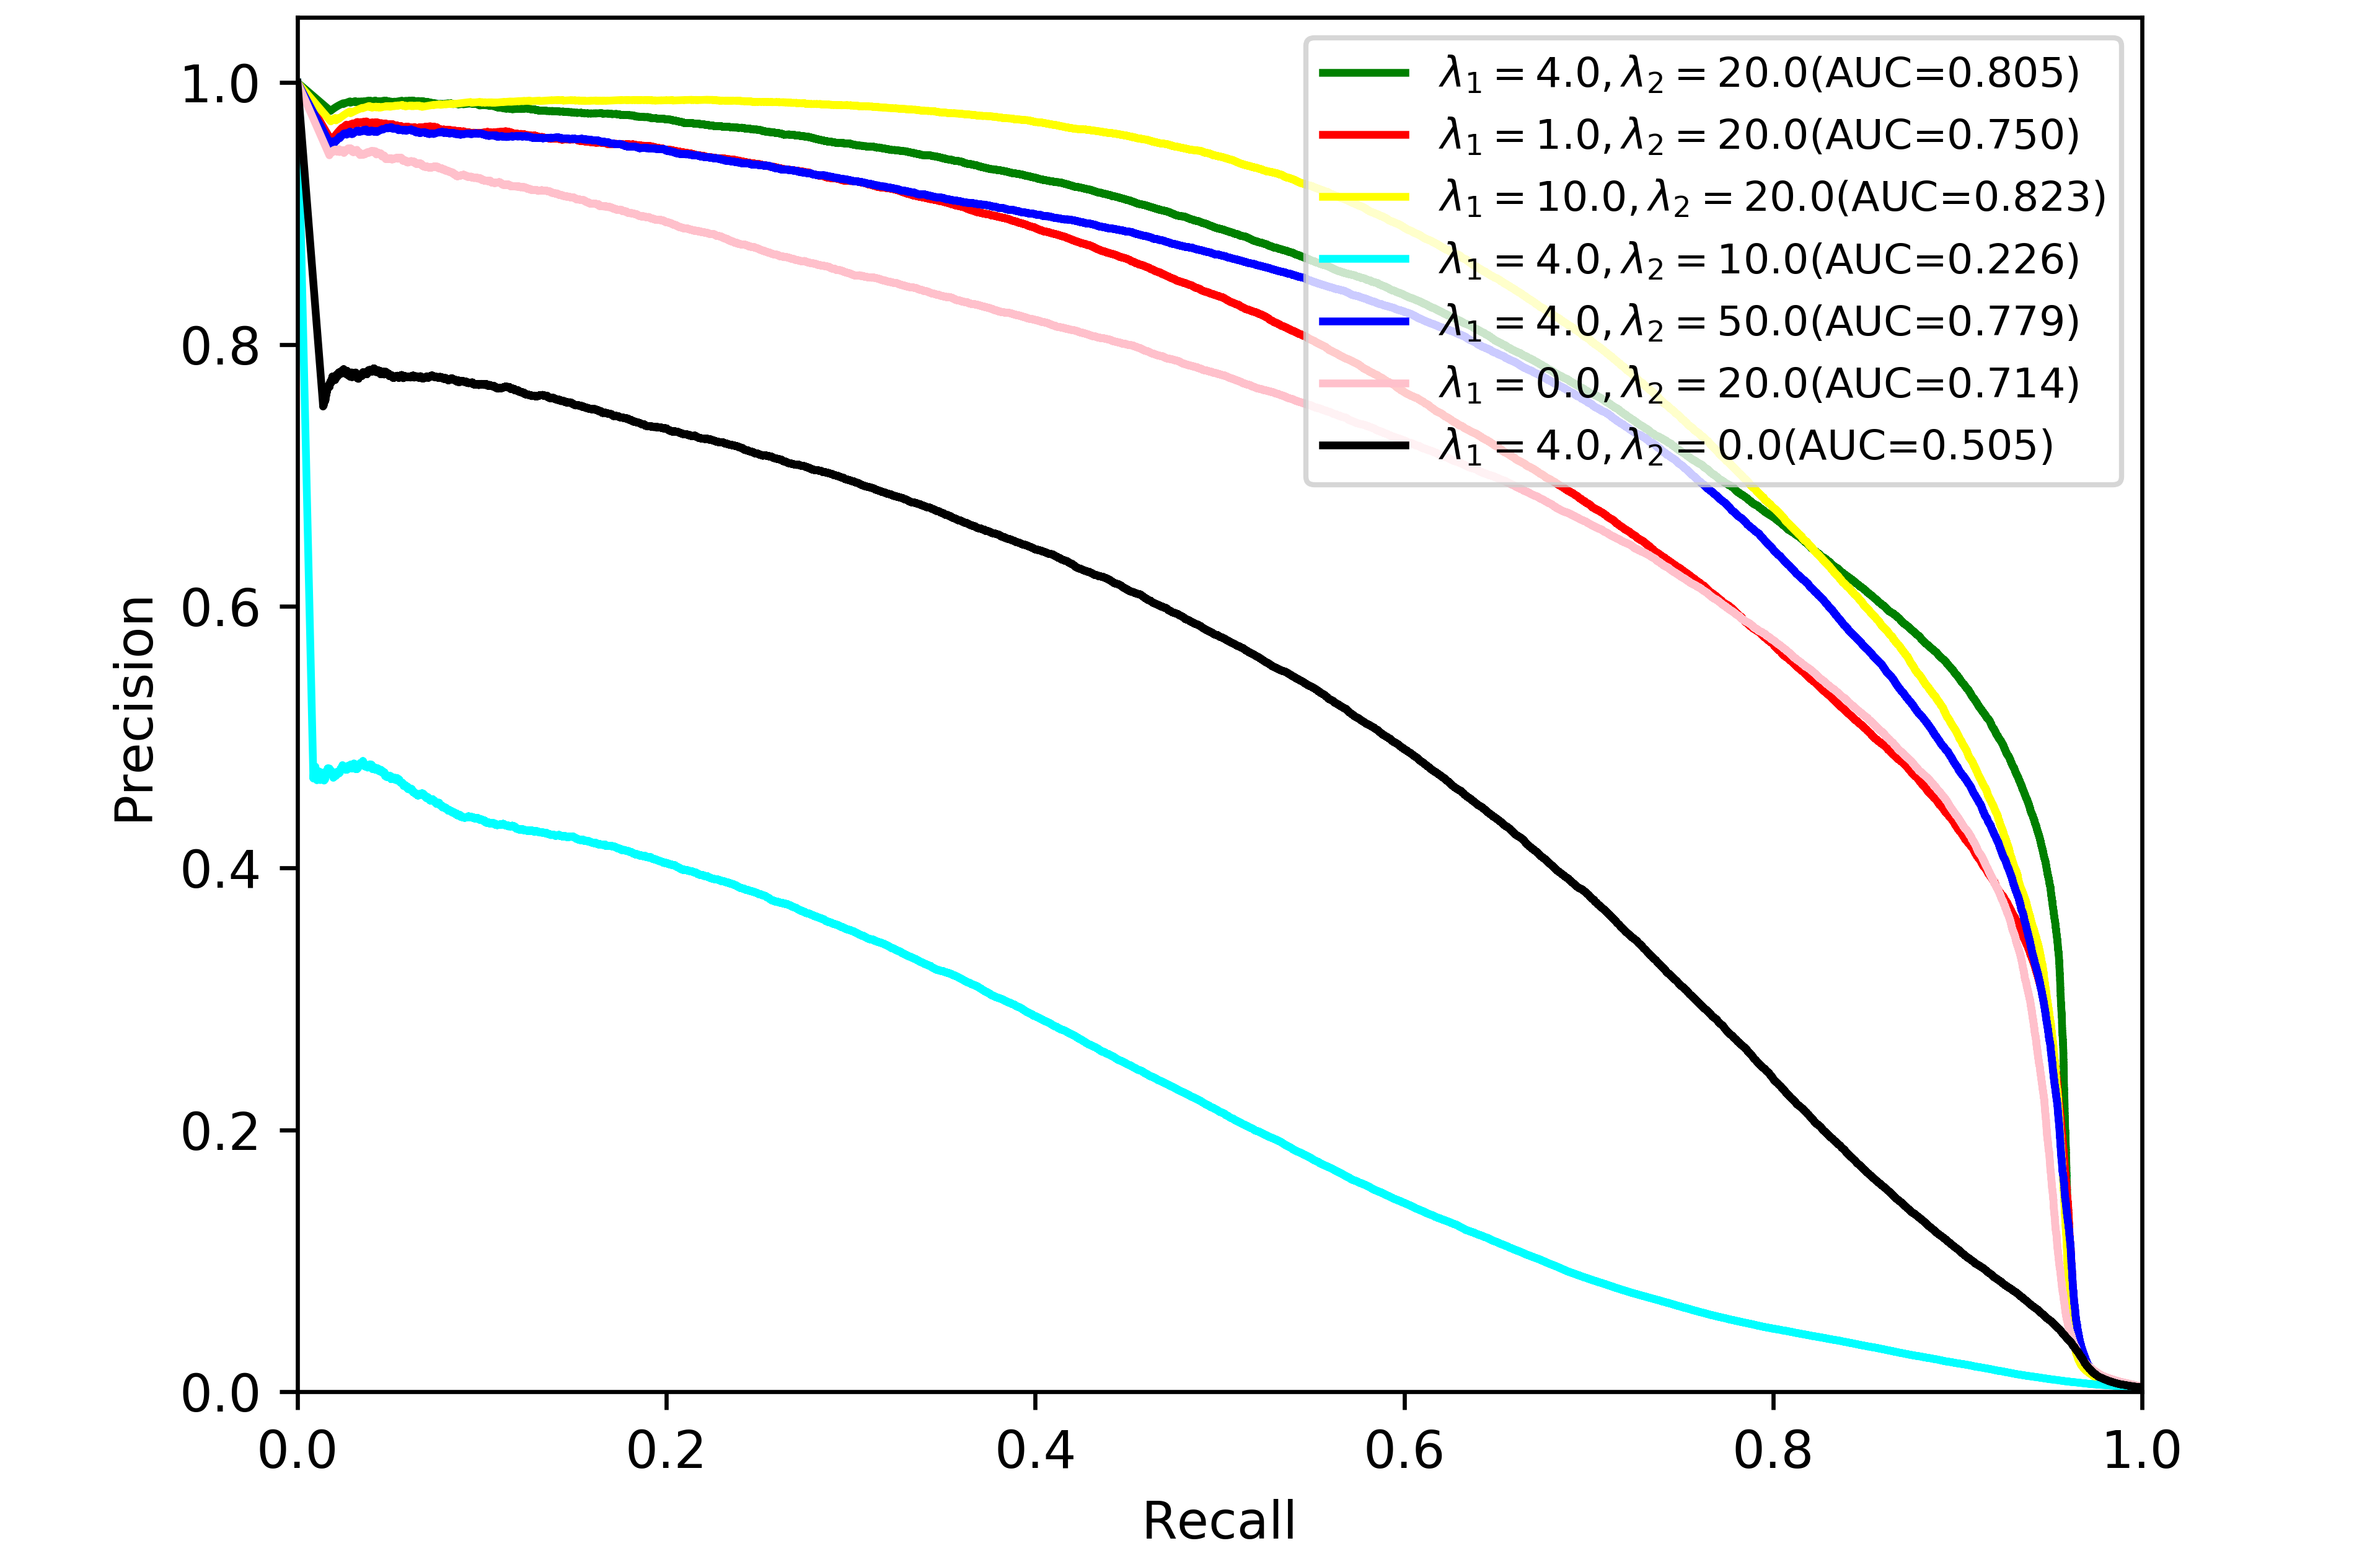
\includegraphics[width=0.6\textwidth]{figure/pr_curve_multi_skin_hyper_paras/CIRCLE_pr_curve.png}
	\caption[不同超参数组合下第三类异常图像上P-R曲线对比]{在多类模拟皮肤病病变数据集上,不同超参数组合下第三类异常图像上P-R曲线对比。} 
	\label{fig:multi_simulate_pr_curve_circle_hyper_paras}
\end{figure}

\begin{table}[H]
	\centering
	\caption[不同超参数组合下三类异常图像P-R曲线的平均AUC分数]{不同超参数组合下三类异常图像P-R曲线的平均AUC分数。}
	\label{tab:simulated_skin_diff_parameters}
%	\resizebox{1.0\textwidth}{!}{
		\begin{tabular}{c|c|c|c|c|c|c|c}
			\toprule[2pt]
			%& $\lambda_{1}=4,\lambda_{2}=20$ & $\lambda_{1}=1, \lambda_{2}=20$& $\lambda_{1}=10, \lambda_{2}=20$&
			
			%$\lambda_{1}=4,\lambda_{2}=10$ & $\lambda_{1}=4,\lambda_{2}=50$ &
			%$\lambda_{1}=0,\lambda_{2}=20$ &
			%$\lambda_{1}=4, \lambda_{2}=0$\\
			超参& $\lambda_{1}=4,$ & $\lambda_{1}=1,$& $\lambda_{1}=10,$&
			$\lambda_{1}=4,$ & $\lambda_{1}=4,$ &
			$\lambda_{1}=0,$ &
			$\lambda_{1}=4,$\\
			组合		  & 
			$\lambda_{2}=20$ & $\lambda_{2}=20$ &
			$\lambda_{2}=20$ & $\lambda_{2}=10$ & $\lambda_{2}=50$ &
			$\lambda_{2}=20$&
			$\lambda_{2}=0$ \\
			\midrule[2pt]
			%第一类异常	& $\textbf{0.236}$ &	$0.135 $ & $0.207$ & $0.084$ & $0.194$& $0.149$ &	$0.176$ \\\hline

			%第二类异常	& $\textbf{0.962}$ &	$0.884 $ & $0.946$ & $0.627$ & $0.910$& $0.847$ & $0.644$	 \\\hline

			%第三类异常	& $0.805$ &	$0.750 $ & $\textbf{0.823}$ & $0.226$ & $0.779$& $0.714$ & $0.505$	 \\\hline

			平均AUC	& $\textbf{0.668}$ &	$0.590 $ & $0.659$ & $0.312$ & $0.628$& $0.570$ &	$0.442$ \\
			\bottomrule[2pt]
		\end{tabular}
%	}
\end{table}
\section{本章小结}
本章主要将本文提出的方法由二类问题推广到多类问题,在此过程中,本文对原始二类模型进行了相关改进,比如,将二类交叉熵损失函数替换成多类交叉熵损失函数、将所有异常类看成判别器的假图像输入端等,以最小的代价实现二类问题到多类问题的扩展,并在多类模拟皮肤病病变数据集上进行了相关实验评估,与CAM和Grad-CAM相比,分别从定性分析(热图)和定量分析(P-R曲线及其AUC)两个角度直接说明本文提出的模型能够更精确地定位疾病标记物,即使疾病标记物广泛分布在异常图像中。本文还分别从额外训练的CNN分类器角度和本文提出的模型本身的判别器角度再次间接地证明了上述结论。最后,为了说明本文提出的方法的超参数鲁棒性,本文还对不同超参数$\lambda_{1}$和$\lambda_{2}$组合进行了测试。到此,本文所有实验内容叙述完毕。在接下来一章中,我们将对本文工作进行总结,并对将来的研究方向进行展望。

